%%%%%%%%%%%%%%%%%%%%%%%%%%%%%%%%%%%%%%%%%%%%%%%%%%%%%%%%%%%%%%%%%%%
%%% Documento LaTeX 																						%%%
%%%%%%%%%%%%%%%%%%%%%%%%%%%%%%%%%%%%%%%%%%%%%%%%%%%%%%%%%%%%%%%%%%%
% T�tulo:	Plantilla de PFC/TFG/TFM
% Autor:  Ignacio Moreno Doblas
% Fecha:  2014-02-01
%%%%%%%%%%%%%%%%%%%%%%%%%%%%%%%%%%%%%%%%%%%%%%%%%%%%%%%%%%%%%%%%%%%
% Compilador: 	MiKTeX 2.9.
%	Modo:					PDFLaTeX.
% Entorno:			TeXnicCenter 2.0 Stable Beta 2.
%%%%%%%%%%%%%%%%%%%%%%%%%%%%%%%%%%%%%%%%%%%%%%%%%%%%%%%%%%%%%%%%%%%

% Pre�mbulo del documento.
%-----------------------------------------------------------------%
% Clase de documento: libro
\documentclass[12pt,a4paper]{book} % article, report, book.

% Pre�mbulo: paquetes, comandos, entornos, estilos y t�tulo de p�gina.
%%%%%%%%%%%%%%%%%%%%%%%%%%%%%%%%%%%%%%%%%%%%%%%%%%%%%%%%%%%%%%%%%%%
%%% Documento LaTeX 																						%%%
%%%%%%%%%%%%%%%%%%%%%%%%%%%%%%%%%%%%%%%%%%%%%%%%%%%%%%%%%%%%%%%%%%%
% T�tulo:	Paquetes
% Autor:  Ignacio Moreno Doblas
% Fecha:  2014-02-01
%%%%%%%%%%%%%%%%%%%%%%%%%%%%%%%%%%%%%%%%%%%%%%%%%%%%%%%%%%%%%%%%%%%
% Tabla de materias:
%	1 Codificaci�n e idioma %
% 2 Matem�ticas y F�sica %
% 3 Gr�ficos%
% 4 Estilo y formato%
%%%%%%%%%%%%%%%%%%%%%%%%%%%%%%%%%%%%%%%%%%%%%%%%%%%%%%%%%%%%%%%%%%%

%1 Codificaci�n e idioma%
\usepackage[latin1]{inputenc} %Codificaci�n en latin-1%
\usepackage[spanish]{babel}	%Hyphenation (Guionado) en espa�ol%
\usepackage[T1]{fontenc} %Codificaci�n de fuente%

%2 Matem�ticas y F�sica %
% Importante para ecuaciones, magnitudes y unidades%
\usepackage{amssymb,amsmath,latexsym,amsfonts} % paquetes est�ndar%
\usepackage[squaren]{SIunits} %Paquete para magnitudes y unidades f�sicas%
\usepackage{ifthen} %sentencias if y while%

%3 Gr�ficos%
\usepackage{graphics,graphicx} %paquetes gr�ficos est�ndar%
\usepackage{wrapfig} %paquete para gr�fica lateral%
\usepackage[rflt]{floatflt} %figuras flotantes%
	% \begin{floatingfigure}[r]/[l]{4.5cm}
	% \end{floatingfigure}
\usepackage{graphpap}	%comando \graphpaper en el entorno picture%

%4 Estilo y formato%
\usepackage{fancyhdr}	%cabeceras y pies mejor que con \pagestyle{}%
\usepackage{titlesec,titletoc} %Formateo de secciones y t�tulos%
\raggedbottom %Para fragmentar versos en varias p�ginas%
\usepackage{makeidx} %MakeIndex%
%\usepackage{showidx} % Hace que cada comando \index se imprima en la p�gina donde se ha puesto (�til para corregir los �ndices)
\usepackage{alltt} % Define el environment alltt, como verbatim, excepto que \, { y } tienen su significado normal. Se describe en el fichero alltt.dtx.
\usepackage[pdftex,bookmarksnumbered,hidelinks]{hyperref} %hyper-references%
\usepackage{minitoc} % Para poner tablas de contenido en cada cap�tulo.
\usepackage{listings} % Para escribir piezas de c�digo C, Python, etc. %
%listings configuration
\lstset{
  language=Python, %Puede ser C, C++, Java, etc.
  showstringspaces=false,
  formfeed=\newpage,
  tabsize=4,
  commentstyle=\itshape,
  basicstyle=\ttfamily,
  morekeywords={models, lambda, forms}
}

\usepackage{tipa} % tipograf�a IPA (International Phonetic Alphabet)
\usepackage{longtable} %Entorno Longtable, fracciona tablas a lo largo de p�ginas%
\usepackage{colortbl}
\usepackage{acronym}  %Para expandir autom�ticamente los acr�nimos
%%%%%%%%%%%%%%%%%%%%%%%%%%%%%%%%%%%%%%%%%%%%%%%%%%%%%%%%%%%%%%%%%%%
%%% Documento LaTeX 																						%%%
%%%%%%%%%%%%%%%%%%%%%%%%%%%%%%%%%%%%%%%%%%%%%%%%%%%%%%%%%%%%%%%%%%%
% T�tulo:	Comandos
% Autor:  Ignacio Moreno Doblas
% Fecha:  2014-02-01
%%%%%%%%%%%%%%%%%%%%%%%%%%%%%%%%%%%%%%%%%%%%%%%%%%%%%%%%%%%%%%%%%%%
% Tabla de materias:
% 1 Informaci�n del Documento %
% 2 Comandos a nivel de texto %
% 3 Comandos a nivel de entorno %
% 4 Comandos a nivel de p�gina y secci�n %
% 5 Otros comandos %
%%%%%%%%%%%%%%%%%%%%%%%%%%%%%%%%%%%%%%%%%%%%%%%%%%%%%%%%%%%%%%%%%%%

% 1 Informaci�n del Documento %
\newcommand{\pfctitlename}{T�tulo del Proyecto fin de Carrera}
\newcommand{\pfcauthorname}{Nombre del autor}
\newcommand{\pfctutorname}{Nombre del tutor}
\newcommand{\pfcanno}{a�o de publicaci�n}

% 2 Comandos a nivel de texto %
\newcommand{\R}{\textsuperscript{\textregistered}}	%S�mbolo registrado%
\newcommand{\C}{\textsuperscript{\copyright}}	%S�mbolo Copyright%
\newcommand{\TM}{\texttrademark} %S�mbolo Trade Mark (marca comercial)%

% 2.1 Comandos abreviatura %
\newcommand{\tit}{\textit} %Fuente cursiva (it�lica)%
\newcommand{\tbf}{\textbf} %Fuente negrita%
\newcommand{\ttw}[1]{\texttt{#1}} %Fuente m�quina de escribir (typewriter)%
%Combinaci�n%
\newcommand{\textittt}[1]{\textit{\texttt{#1}}} %it�lica y typewriter%
\newcommand{\textittw}{\textittt} % Otra forma de escribirlo.
\newcommand{\tittw}{\textittw} %Shortened%
\newcommand{\tbftw}[1]{\tbf{\ttw{#1}}}

%Crea una nueva l�nea y la indenta sin crear interlineado extra.
\newcommand{\nli}{\\ \indent} 

%Para escribir un correo electr�nico%
\newcommand{\mailto}[1]{\href{mailto:#1}{#1}}

% Si vas a hacer un uso b�sico de \index (entradas en el �ndice de s�lo un nivel, sin formatos especiales, etc.), define la orden
\newcommand{\miindex}[1]{#1\index{#1}}

\newcommand{\hs}{\hspace} % Abreviatura espacio horizontal
\newcommand{\vs}{\vspace} % Abreviatura espacio vertical

% Abreviaturas para los conjuntos de n�meros m�s comunes.
\newcommand{\realnumbers}{\mathbb R}
\newcommand{\naturalnumbers}{\mathbb N}
\newcommand{\integernumbers}{\mathbb Z}
\newcommand{\rationalnumbers}{\mathbb Q}
\newcommand{\complexnumbers}{\mathbb R}
\newcommand{\irrationalnumbers}{\mathbb I}

% Doble barra sobre una letra (para expresar las matrices).
\newcommand{\doublebar}[1]{\bar{\bar{#1}}} 
% Ej: \vector(y) = \doublebar(A) \vector(x) (Stma. lineal de ec.)

% 3 Comandos a nivel de entorno %
\newcommand{\benu}{\begin{enu}} % Begin enumerate
\newcommand{\eenu}{\end{enu}} 	% End enumeration

%Comando para escribir c�digo Python
\newcommand{\code}[3]{
  %\hrulefill
  %\subsection*{#1}
  %\subsubsection{#1}
  \lstinputlisting{#2}
  %#1\\
  \begin{table}[h!]
  	\centering
  	\caption{#1}
  	\label{#3}
  \end{table}
  \vspace{2em}
}

% 4 Comandos a nivel de p�gina y secci�n %
%Crea p�gina en blanco
\newcommand{\blankpage}{\clearpage{\pagestyle{empty}\cleardoublepage}}

% Versi�n x del comando section: sin numeraci�n pero s� aparece en la tabla de contenidos.
\newcommand{\sectionx}[1]{
	\section*{#1}
	\addcontentsline{toc}{section}{#1}
}

% Versi�n y del comando section: sin numeraci�n y NO aparece en la tabla de contenidos.
\newcommand{\sectiony}[1]{
	\section*{#1}
}

% Versi�n x del comando chapter: sin numeraci�n pero s�  aparece en la tabla de contenidos.
\newcommand{\chapterx}[1]{
	\chapter*{#1}
	%\addcontentsline{toc}{chapter}{#1} %Caused by minitoc package%
	\addstarredchapter{#1} %For minitoc package%
}

% substituto del comando \chapter: incluye estilo de p�gina.
\newcommand{\chapterbegin}[1]%
	{%
		\pagestyle{fancy}
		\fancyhead[LE,RO]{\thepage}
		\fancyhead[LO]{Cap�tulo \thechapter. #1}
		%\fancyhead[RE]{Parte \thepart \rightmark} %
		\fancyhead[RE]{\nouppercase{\rightmark}} %
				
		\chapter{#1}
	}

% Versi�n x del comando \chapterbegin: sin numeraci�n y aparece en la tabla de contenidos.
\newcommand{\chapterbeginx}[1]%
	{%
		\pagestyle{fancy}
		\fancyhead[RO,LE]{\thepage}
		\fancyhead[RE,LO]{#1}
		%\fancyhead[LO]{Chapter \thechapter}
		%\fancyhead[RE]{Part \thepart} %
		
		\chapterx{#1}
	}

%Fin de cap�tulo
\newcommand{\chapterend}{\pagestyle{empty}\cleardoublepage \thispagestyle{empty}}
%Si fuera un art�culo en lugar un libro, \clearpage en lugar de \cleardoublepage

% 5 Otros comandos %
%\let\Oldpart\part
%\newcommand{\parttitle}{}
%\renewcommand{part}[1]{\Oldpart{#1}\renewcommand{\parttitle}{#1}} %Header customization%

%Cambiar el t�tulo �ndice de cap�tulo a ``Contenido''.
\renewcommand{\mtctitle}{Contenido}

\dominitoc % Para tablas de contenidos por cap�tulo.

\addto{\captionsspanish}{
	\renewcommand{\listtablename}{�ndice de Tablas}
	\renewcommand{\tablename}{Tabla} } % Por ejemplo, modificar el nombre de 'Cuadro' a 'Tabla'.

\addto{\captionsspanish}{
	\renewcommand{\contentsname}{�ndice} }

%Si se desea cambiar el tipo de letra a Arial
% por cualquier raz�n, descomentar las siguientes
% dos l�neas
%\renewcommand{\rmdefault}{phv} % Arial
%\renewcommand{\sfdefault}{phv} % Arial
	
%\addto{\captionsspanish}{
%	\renewcommand{\partname}{Fase} }

%\addto{\captionsspanish}{%
%    \renewcommand{\refname}{\vspace{-4.5ex}}} % Para que no aparezca el texto 'referencias' en la bibliograf�a.

% Modifica el interlineado
%\renewcommand{\baselinestretch}{1.5}
%%%%%%%%%%%%%%%%%%%%%%%%%%%%%%%%%%%%%%%%%%%%%%%%%%%%%%%%%%%%%%%%%%%
%%% Documento LaTeX 																						%%%
%%%%%%%%%%%%%%%%%%%%%%%%%%%%%%%%%%%%%%%%%%%%%%%%%%%%%%%%%%%%%%%%%%%
% T�tulo:	Entornos
% Autor:  Ignacio Moreno Doblas
% Fecha:  2014-02-01
%%%%%%%%%%%%%%%%%%%%%%%%%%%%%%%%%%%%%%%%%%%%%%%%%%%%%%%%%%%%%%%%%%%
% Tabla de materias:
%--------------------%
% 1 dobleindent
% 2 izqindent
% 3 dobleindentx
% 4 ite
% 5 descript
% 6 enu
% 7 itemization
% 8 sinopsis
%%%%%%%%%%%%%%%%%%%%%%%
% Para conocer los par�metros de dise�o de las listas, tales como
%  los m�rgenes izquierdo, derechos y los diferentes saltos,
%  v�ase el archivo ``List layout.png'' que acompa�a esta plantilla.
% As� se conocer� mejor c�mo adaptar un entorno seg�n los requisitos 
%  del usuario.

%%%%%%%%%%%%%%%%%%%%%%%
% Definici�n de longitudes para usar en los entornos:
%
% Normal parskip.
\newlength{\parskipenv}
\setlength{\parskipenv}{\parskip}

\newlength{\parindentenv}
\setlength{\parindentenv}{\parindent}
%%%%%%%%%%%%%%%%%%%%%%%

% 1 dobleindent
%El entorno dobleindent est� pensando para escribir p�rrafos con doble indentaci�n a cada lado.
%Tiene dos par�metros de entrada con las distancias medidas desde los m�rgenes de p�gina.

\newenvironment{dobleindent}[2]
	%Comienzo de nuevo entorno%
	{
	\begin{list}
		{}
		{
		% Left and right margins:
		\leftmargin = #1 
		\rightmargin = #2
		%
		% Separation from preceding and following text:
		\topsep = 0ex
		\partopsep = 0ex
		\parsep = \parskipenv
		%
		% Indentation for paragraphs:
		\itemsep = \parskipenv
		\itemindent = \parindentenv
		\listparindent = \itemindent
		%
		% Horizontal separation from label:
		\labelsep = 1ex
		\settowidth{\labelwidth}{0cm}
		}
		
		 \item}
	% End new env
	{\end{list}}

%%%%%%%%%%%%%%%%%%%%%%%%%%%%%
%2 izqindent
% El entorno izqindent s�lo crea un p�rrafo indentado a la izquierda.
\newenvironment{izqindent}[1]
{
\begin{dobleindent}{#1}{0cm}
}
{
\end{dobleindent}
}

%%%%%%%%%%%%%%%%%%%%%%%%%%%%%
% 3 dobleindentx
% El entorno dobleindentx es una variaci�n del dobleindent usando leftskip y rightskip.
% Aunque es m�s limitado, tambi�n se puede usar.
\newenvironment{dobleindentx}[2] % S�lo funciona en modo paragraph
{ % Preamble
  \leftskip = #1
  \rightskip = #2
}
{ % Postamble
\leftskip = 0cm
\rightskip = 0cm
}

%%%%%%%%%%%%%%%%%%%%%%%%%%%%%
% 4 ite
% El entorno ite es una modificaci�n del entorno itemize est�ndar de \LaTeX. Puede usarse o modificarse si el usuario lo desea.
% Tambi�n puede parametrizarse el entorno enumerate o description de forma equivalente.
\newenvironment{ite}
	{
		\begin{izqindent}{\parindent}
		\hspace{-\parindent} 	% compensaci�n del sangrado que introduce el entorno.
		\vspace{-1.0\parskip}	% compensaci�n del \parskip que introduce el entorno.
		\vspace{-\baselineskip}	% compensaci�n por la l�nea que introduce el entorno.
		\begin{itemize}
	}
	{
		\end{itemize}
		\end{izqindent}
	}

%%%%%%%%%%%%%%%%%%%%%5
% commando stdformat para formatear los entornos descript, enu y itemization.
\newcommand{\stdformat}
	{% Declarations for format presentation.
		%		  
		% Separation from preceding and following text:
		\setlength{\topsep}{0ex}%
		\setlength{\partopsep}{0ex} %
		%
		% Horizontal separation from label:
		\labelsep = 1ex
		\setlength{\labelwidth}{0ex}
		%
		%	Left and right margins:	
		\setlength{\leftmargin}{1cm}%
		\addtolength{\leftmargin}{\labelsep}
		\setlength{\rightmargin}{0ex}
		%  
		% Indentation for paragraphs:
		\setlength{\itemindent}{-\leftmargin}%
		\addtolength{\itemindent}{1ex}
		\setlength{\listparindent}{\parindent}%
		%		
		% Separation between paragraphs.
		\setlength{\parsep}{\parskipenv}% 
		\setlength{\itemsep}{1ex}
	}

%%%%%%%%%%%%%%%%%%%%%%%%%%%%%
% 5 descript

\newenvironment{descript}
	% Beginning new env def.
	{
		\begin{list}
			{} % No default label for \item.
			{
				% Declarations for format presentation.
				\stdformat
				%
				\renewcommand{\makelabel}[1]{\normalfont\bfseries##1\hfil}
			}
	}
	% Ending new env def.
	{
		\hspace*{\fill} \\ \end{list}
	} % Se introduce un salto de l�nea para que el texto siguiente est� separado.
%END newenvironment{descript}

%%%%%%%%%%%%%%%%%%%%%%%%%%%%%
% 6 enu
\newcounter{itemnumber} % Counter for the environment.

\newenvironment{enu}
	% Beginning new env def.
	{
		\begin{list}
		{
			\raggedleft \arabic{itemnumber}
		}
		{
			\usecounter{itemnumber}
			\stdformat
		}
	}
	{
		\end{list}
	}

%%%%%%%%%%%%%%%%%%%%%%%%%%%%%
% 7 itemization
\newenvironment{itemization}
	% Beginning new env def.
	{
		\begin{list}
			{$\bullet$} % No default label for \item.
			{
				% Declarations for format presentation.
				\stdformat
			}
	}
	% Ending new env def.
	{
		\end{list}
	}


%%%%%%%%%%%%%%%%%%%%%%%%%%%%%
% 8 sinopsis
\newenvironment{sinopsis}{%[1]{
	\sectiony{Sinopsis}
	%\label{#1}
} {
	\pagebreak
}
%%%%%%%%%%%%%%%%%%%%%%%%%%%%%%%%%%%%%%%%%%%%%%%%%%%%%%%%%%%%%%%%%%%
%%% Documento LaTeX 																						%%%
%%%%%%%%%%%%%%%%%%%%%%%%%%%%%%%%%%%%%%%%%%%%%%%%%%%%%%%%%%%%%%%%%%%
% T�tulo:	Par�metros de estilo
% Autor:  Ignacio Moreno Doblas
% Fecha:  2014-02-01
%%%%%%%%%%%%%%%%%%%%%%%%%%%%%%%%%%%%%%%%%%%%%%%%%%%%%%%%%%%%%%%%%%%
% Tabla de materias:
%--------------------%
% 1 M�rgenes de p�gina
%%%%%%%%%%%%%%%%%%%%%%%
% Para conocer los par�metros de dise�o de p�ginas, tales como
%  los m�rgenes izquierdo, derecho, anchura de p�gina, etc.
%  v�ase el archivo ``Page layout.png'' que acompa�a esta plantilla.
% As� se conocer� mejor c�mo adaptar el documento seg�n los 
%  requisitos del usuario.

% 1 M�rgenes de p�gina
%-------------------------------%
% Par�metros de estilo de p�gina.
% DIN A4: 29.7 cm x 21 cm
%		�rea neta: 3 cm + 3 cm + 15 cm.
%
% Definici�n de m�rgenes de p�gina
%  even para p�ginas pares
%  odd  para p�ginas impares
\newlength{\realoddsidemargin}	  % \oddsidemargin menos 1 in.
\newlength{\realevensidemargin}		% \evensidemargin menos 1 in.
\newlength{\realtopmargin}				% \topmargin menos 1 in.
%
% Asignaci�n de m�rgenes de p�gina
% ASIGNESE en caso de querer cambiarlo
\setlength{\realtopmargin}{2cm}			% REAL top margin.
\setlength{\realoddsidemargin}{3cm}		% REAL oddside margin.
\setlength{\realevensidemargin}{3cm}	% REAL evenside margin.
\setlength{\hoffset}{0cm}
\setlength{\voffset}{0cm}
%
% Substracci�n de 1 pulgada de compensaci�n
%  (v�ase ``Page Layout.png'' para m�s informaci�n)
\addtolength{\realoddsidemargin}{-1in}	% 1 inch = 2.54 cm.
\addtolength{\realevensidemargin}{-1in}
\addtolength{\realtopmargin}{-1in}
%
% Asignaci�n de anchuras y m�rgenes
% No hay notas al margen
\setlength{\marginparsep}{0cm} % No van a existir notas al margen
\setlength{\marginparwidth}{0cm} % No van a existir notas al margen
%
% Asignaci�n de anchura de texto
\setlength{\textwidth}{15cm}	% Anchura neta del texto (globalmente).
%
% Asignaci�n de m�rgenes par, impar y en altura
\setlength{\oddsidemargin}{\realoddsidemargin}	% odd-page left margin (global).
\setlength{\evensidemargin}{\realoddsidemargin}	% even-page left margin (global).
\setlength{\topmargin}{\realtopmargin}					% top margin (Global).

% Se puede usar tambi�n el paquete chngpage.

%%%%%%%%%%%%%%%%%%%%%%%%%%%%%%%%%%%%%%%%%%%%%%%%%%%%%%%%%%%%%%%%%%
%		1 Length commands.					%
%-------------------------------%
% Defines new length command (e.g., \newlength{\gnat}}
%	\newlength{}
%
% Set lenght to a value.
%	\setlength{\gnat}{length}
%	\addtolength{}{}
%
% Sets the value of a length command equal to the width of a specified piece of text; e.g., \settowidth{\parindent}{\em small}.
%	\settowidth{}{}
% Set the value of a height. e.g., \settoheight{\parskip}{Gnu}
%	\settoheight{}{}
% Set the value that extends below the line. e.g., \settodepth{\parskip}{gnu}.
%	\settodepth{}{}
%
% To multiply a length, write: 7.0\gnat = \gnat * 7.0
%%%%%%%%%%%%%%%%%%%%%%%%%%%%%%%%%%%%%%%%%%%%%%%%%%%%%%%%%%%%%%%%%%

%Comando para crear glosario (index en ingl�s)
\makeindex


% Document body.
%-------------------------------------------------------------------%
\begin{document}

% Formato de documento hasta el cap�tulo 1 (sin incluirlo)
\frontmatter

%% T�tulo y autor del proyecto
%%Rellenar con el nombre real del autor, t�tulo, tutor y a�o.
%%El departamento del tutor se escribe una vez en el Resumen del PFC
%\renewcommand{\pfcauthorname}{Nombre del autor}
%\renewcommand{\pfctitlename}{T�tulo del proyecto}
%\renewcommand{\pfctutorname}{Nombre del tutor}
%\renewcommand{\pfcanno}{2014}

% Los tres ficheros siguientes solamente deben descomentarse
%  en el caso de ser un PFC del plan a extinguir.
% En los nuevos t�tulos de grado, no exiten la portada, la calificaci�n 
%  ni el Resumen del PFC.
% Estos tres documentos deben tomarse de la web de la ETSIT.
%
% Portada.
%%%% Tipos de portada %%%
%	1. \maketitle
%	2. titlepage
%%%%%%%%%%%%%%%%%%%%%%%%

%	1. \maketitle
%%%%%%%%%%%%%%%%%%%%%%%%
%\maketitle
%\thispagestyle{empty}

%	2. titlepage
%%%%%%%%%%%%%%%%%%%%%%%%
\begin{titlepage}
	\begin{center}
		\Large {\textsc{\textsf{
		Escuela T�cnica Superior de\\
		Ingenier�a de Telecomunicaci�n\\
		Universidad de M�laga}	}}
	\end{center}
	
	\bigskip
	
	\begin{center}
		\begin{tabular}{lcr}
			%
\includegraphics[width=4cm,keepaspectratio]{graphs/EscudoETSIT.jpg} & \hspace{2cm}
			
\includegraphics[width=4cm,keepaspectratio]{graphs/EscudoETSIT.pdf} & \hspace{2cm}
			
\includegraphics[width=4cm,keepaspectratio]{graphs/UnivMalacitana.pdf}
		\end{tabular}
	\end{center}
	
	\bigskip
	
	\begin{center}\Large\textbf{\textsf{PROYECTO FIN DE CARRERA}}\end{center}
	
	\medskip
	
	\begin{center}
		\Huge
		\sffamily\scshape
		\pfctitlename		
	\end{center}
	
	\medskip
	
	\begin{center}
		\Huge
		\scshape%\bfseries
		\textsf{Ingenier�a de Telecomunicaci�n}
	\end{center}
	
	\vfill
	
	{\large M�laga, \pfcanno \hfill \pfcauthorname}
	%\blankpage
\end{titlepage}


% Hoja de calificaci�n
%\thispagestyle{empty}
\begin{center}
	\Large \sffamily \scshape %\bfseries
	Escuela T�cnica Superior de\\
	Ingenier�a de Telecomunicaci�n\\
	Universidad de M�laga
\end{center}

	{\bfseries Titulaci�n: Ingenier�a de Telecomunicaci�n}\\[3ex]

	\noindent Reunido el tribunal examinador en el d�a de la fecha, constituido por:\\[3ex]
	\textbf{D./D�.~}\hrulefill\\[3ex]
	\textbf{D./D�.~}\hrulefill\\[3ex]
	\textbf{D./D�.~}\hrulefill\\[3ex]
	
	para juzgar el Proyecto Fin de Carrera titulado:\noindent 
	
\begin{center}
	\large \bfseries \pfctitlename
\end{center}

\noindent del alumno \tit{D./D�.~\pfcauthorname}

\noindent dirigido por \tit{D./D�.~\pfctutorname}

\bigskip

	\noindent ACORD� POR \hrulefill OTORGAR LA\\[3ex]%\rule{3cm}{0.1mm} otorgar la\\[3ex]
	CALIFICACI�N DE\hrulefill\\[3ex]
	
	%\hrulefill\\[3ex]
	
	\noindent y, para que conste, se extiende firmada por los componentes del tribunal, la presente diligencia.
	
	\bigskip

\hfill M�laga, a \rule{1cm}{0.1mm} de \rule{1cm}{0.1mm} de \rule{0.7cm}{0.1mm}

\vfill

\begin{center}
	\begin{tabular}{ccc}
	El Presidente: & El Vocal: & El Secretario:\\[2cm]
	Fdo.:\rule{3cm}{0.1mm} & Fdo.:\rule{3cm}{0.1mm} & Fdo.:\rule{3cm}{0.1mm}	
	\end{tabular}
\end{center}

\blankpage

% Resumen del proyecto (formulario)
%%%%%%%%%%%%%%%%%%%%%%%%%%%%%%%%%%%
% P�gina de resumen del proyecto %
%%%%%%%%%%%%%%%%%%%%%%%%%%%%%%%%%%

\thispagestyle{empty}
\begin{center}
	\Large \sffamily
	Universidad de M�laga\\
	Escuela T�cnica Superior de Ingenier�a de\\
	Telecomunicaci�n
\end{center}

\bigskip

\begin{center}
	\Huge\scshape
	\pfctitlename
\end{center}

\bigskip

\begin{center}
	\textbf{REALIZADO POR}\\
	\textsf{\pfcauthorname}
\end{center}

\medskip

\begin{center}
	\textbf{DIRIGIDO POR}\\
	\textsf{\pfctutorname}
\end{center}

\vfill

\begin{minipage}{\textwidth}
\textbf{Dpto. de:} Ingenier�a de Comunicaciones (DIC)

\medskip

\textbf{Palabras clave:} palabras, clave, del, proyecto, separadas, por, coma

\medskip

\textbf{Titulaci�n:} Ingenier�a de Telecomunicaci�n

\medskip

\textbf{Resumen:}
	Aqu� se explica un breve resumen del proyecto, en qu� consiste, cu�l es
su prop�sito, etc.\\
	Puede usarse m�s de un p�rrafo si es necesario.

\begin{center} M�laga, \today\end{center}
\end{minipage}

\blankpage

% Dedicatoria.
%%%%%%%%%%%%%%%%%%%%%%%%%%%%%%%%%%%%%%%%%%%%%%%%%%%%%%%%%%%%%%%%%%%
%%% Documento LaTeX 																						%%%
%%%%%%%%%%%%%%%%%%%%%%%%%%%%%%%%%%%%%%%%%%%%%%%%%%%%%%%%%%%%%%%%%%%
% T�tulo:	Dedicatoria
% Autor:  Ignacio Moreno Doblas
% Fecha:  2014-02-01
%%%%%%%%%%%%%%%%%%%%%%%%%%%%%%%%%%%%%%%%%%%%%%%%%%%%%%%%%%%%%%%%%%%
% Esta plantilla sirve para dedicatoria.

\cleardoublepage
\thispagestyle{empty} % No queremos mostrar ning�n encabezamiento ni pie de p�gina.

\begin{minipage}[c][\textheight][c]{\textwidth} %[pos][height][inner-pos]{width}
\raggedleft %\flushleft

En caso de dedicatoria, \\
se realiza con esta p�gina.\\
No es obligatoria, si bien es recomendable.
hasta luego
\bigskip

\emph{El autor}

\end{minipage}

\blankpage

% Acr�nimos
%%%%%%%%%%%%%%%%%%%%%%%%%%%%%%%%%%%%%%%%%%%%%%%%%%%%%%%%%%%%%%%%%%%
%%% Documento LaTeX 																						%%%
%%%%%%%%%%%%%%%%%%%%%%%%%%%%%%%%%%%%%%%%%%%%%%%%%%%%%%%%%%%%%%%%%%%
% T�tulo:	Lista de acr�nimos
% Autor:  Ignacio Moreno Doblas
% Fecha:  2014-02-01
%%%%%%%%%%%%%%%%%%%%%%%%%%%%%%%%%%%%%%%%%%%%%%%%%%%%%%%%%%%%%%%%%%%

%Lista de acr�nimos 
\chapterbeginx{Acr�nimos}

\begin{acronym}[DLMS/COSEMM]
	
	
	\acro{ADNI}{Alzheimer's Disease Neuroimaging Initiative}
	\acro{AD}{\textit{Alzheimer Disease}}	
	\acro{CMV}{Voto por Mayor�a Complejo}
	\acro{CNN}{Red Neuronal Convolucional}	
	\acro{CSF}{Fluido Cerebro-Espinal}
	\acro{GM}{Materia Gris}
	\acro{PCA}{An�lisis de Componentes Principales}
	\acro{PET}{Tomograf�a por Emisi�n de Positrones}
	\acro{MCI}{\textit{Mild Cognitive Impairment}}
	\acro{MRI}{Im�gen Resonancia Magn�tica}
	\acro{NC}{\textit{Normal Control}}
	\acro{ROI}{R�giones de Interes}
	\acro{SGD}{Descenso en Gradiente Estoc�stico}
    \acro{SMV}{Voto por Mayor�a Simple}
    \acro{SVM}{M�quina de Vectores de Soporte}
	\acro{VAE}{Autoencoder Variacional}
	\acro{CVAE}{Autoencoder Variacional Convolucional}
	\acro{WM}{Materia Blanca}
\end{acronym}

\chapterend

% Tabla de contenidos, figuras y tablas.
%%%%%%%%%%%%%%%%%%%%%%%%%%%%%%%%%%%%%%%%%%%%%%%%%%%%%%%%%%%%%%%%%%%
%%% Documento LaTeX 																						%%%
%%%%%%%%%%%%%%%%%%%%%%%%%%%%%%%%%%%%%%%%%%%%%%%%%%%%%%%%%%%%%%%%%%%
% Título:	Índice (Tabla de contenidos)
% Autor:  Ignacio Moreno Doblas
% Fecha:  2014-02-01
%%%%%%%%%%%%%%%%%%%%%%%%%%%%%%%%%%%%%%%%%%%%%%%%%%%%%%%%%%%%%%%%%%%

%\pagestyle{fancy}

%\dominitoc %Este comando es para el índice por capítulo%

\tableofcontents

%\fancyhead[RO,LE]{\roman{page}} %El contador page no lleva \
%\fancyhead[LO,RE]{Tabla de Contenidos}
%\fancyhead[RE,LO]{\nouppercase{\rightmark}}
%\fancyfoot[C]{}

%\dottedcontents{part}[1em]{\bfseries \large Part }{0em}{1pc}
%\dottedcontents{chapter}[0.5cm]{\ }{1em}{1pc}
%\titlecontents{chapter}[2em]{}{Chapter \thecontentslabel}{}{\\}
%\dottedcontents{chapter}[2.5em]{Chapter }{0em}{1pc}

\chapterend

%%%%%%%%%%%%%%%%%%%%%%%%%%%%%%%%%%%%%%%%%%%%%%%%%%%%%%%%%%%%%%%%%%%
%%% Documento LaTeX 																						%%%
%%%%%%%%%%%%%%%%%%%%%%%%%%%%%%%%%%%%%%%%%%%%%%%%%%%%%%%%%%%%%%%%%%%
% Título:	Índice de Figuras (Tabla de Figuras)
% Autor:  Ignacio Moreno Doblas
% Fecha:  2014-02-01
%%%%%%%%%%%%%%%%%%%%%%%%%%%%%%%%%%%%%%%%%%%%%%%%%%%%%%%%%%%%%%%%%%%

\pagestyle{fancy}

\listoffigures
\fancyhead[RO,LE]{\roman{page}} %El contador page no lleva \

\fancyhead[RE,LO]{\nouppercase{\rightmark}}

\chapterend
%%%%%%%%%%%%%%%%%%%%%%%%%%%%%%%%%%%%%%%%%%%%%%%%%%%%%%%%%%%%%%%%%%%
%%% Documento LaTeX 																						%%%
%%%%%%%%%%%%%%%%%%%%%%%%%%%%%%%%%%%%%%%%%%%%%%%%%%%%%%%%%%%%%%%%%%%
% Título:	Índice de Tablas (Tabla de Tablas)
% Autor:  Ignacio Moreno Doblas
% Fecha:  2014-02-01
%%%%%%%%%%%%%%%%%%%%%%%%%%%%%%%%%%%%%%%%%%%%%%%%%%%%%%%%%%%%%%%%%%%

\pagestyle{fancy}

\listoftables

\fancyhead[RO,LE]{\roman{page}}
\fancyhead[RE,LO]{\nouppercase{\rightmark}}

\chapterend

% Formato de documento durante los cap�tulos.
\mainmatter

% Pr�logo.
%%%%%%%%%%%%%%%%%%%%%%%%%%%%%%%%%%%%%%%%%%%%%%%%%%%%%%%%%%%%%%%%%%%
%%% Documento LaTeX 																						%%%
%%%%%%%%%%%%%%%%%%%%%%%%%%%%%%%%%%%%%%%%%%%%%%%%%%%%%%%%%%%%%%%%%%%
% T�tulo:	Pr�logo
% Autor:  Ignacio Moreno Doblas
% Fecha:  2014-02-01
%%%%%%%%%%%%%%%%%%%%%%%%%%%%%%%%%%%%%%%%%%%%%%%%%%%%%%%%%%%%%%%%%%%

\chapterbeginx{Pr�logo}

%\minitoc
	Aqu� debe escribirse el pr�logo del proyecto fin de carrera.
	\medskip
	
	La calidad en la presentaci�n de los textos y las flexibilidad de \LaTeX\ me llevaron a aprenderlo, a pesar de su dif�cil curva de aprendizaje.\nli
	Espero que esta plantilla ayude notablemente a suavizar este inconveniente.
	
	Quiero agradecer a las personas que han colaborado en la realizaci�n de esta plantilla \LaTeX. Es un sistema muy r�pido y c�modo en la generaci�n de este tipo de documentos t�cnicos y su lectura es francamente agradable.
	
	Animo a todo el mundo a utilizarlo.
	
	Desde la p�gina de la escuela hay disponible tambi�n un \miindex{manual de estilo} para ayudar en la redacci�n y el acabado del proyecto.
	Puede consultarse en~\cite{GuiaEstilo}~\footnote{
		\url{http://www.uma.es/media/files/Manual_de_Estilo_TFG_ETSIT.pdf}
	}.

	Tambi�n ser�a interesante hacer dos manuales m�s: 
\begin{itemize}
	\item{Uno de \LaTeX, que explique con m�s detalle c�mo utilizar este sistema. Aunque en Internet hay muchos disponibles, un manual r�pido y directo suavizar�a a�n m�s la curva de aprendizaje.\nli
		Quiz�, lo m�s importante es que integre todos los elementos que un usuario necesita, ya que normalmente es necesario acudir a varias fuentes y eso suele requerir demasiado tiempo.\nli
		El cap�tulo~\ref{chp:ManLaTeX} contiene informaci�n orientada a un iniciado en este sistema.}
	
	\item{Y otro, que explique herramientas y m�todos �tiles que un proyectando puede necesitar en la elaboraci�n del proyecto, tal como llevar un control de versiones de la documentaci�n o el c�digo fuente desarrollado utilizando Assembla\TM. Este �ltimo manual es interesante tambi�n para muchos j�venes profesionales, especialmente en el �rea de desarrollo de sistemas.}
\end{itemize}

	Me reservo el derecho de hacerlo, dado el escaso tiempo del que dispongo.
	\bigskip
	
	Muchas gracias.

\chapterend

% Capitulos
%%%%%%%%%%%%%%%%%%%%%%%%%%%%%%%%%%%%%%%%%%%%%%%%%%%%%%%%%%%%%%%%%%%
%%% Documento LaTeX 																						%%%
%%%%%%%%%%%%%%%%%%%%%%%%%%%%%%%%%%%%%%%%%%%%%%%%%%%%%%%%%%%%%%%%%%%
% T�tulo:		Cap�tulo 1
% Autor:  	Ignacio Moreno Doblas
% Fecha:  	2014-02-01
% Versi�n:	0.5.0
%%%%%%%%%%%%%%%%%%%%%%%%%%%%%%%%%%%%%%%%%%%%%%%%%%%%%%%%%%%%%%%%%%%
\chapterbegin{Introduccion}
%%\minitoc

La demencia engloba un amplio grupo de enfermedades mentales que provocan el deterioro progresivo de las facultades mentales de la persona que la padece tales como la memoria, el aprendizaje, el lenguaje o la orientaci�n. 
\par La enfermedad del Alzheimer (AD) es la forma de demencia mas c�mun en personas de la tercera edad.  La AD es un desorden neurodegenerativeo que afecta a la memoria en primer lugar, y progresivamente al resto de funciones cognitivas, provocando desajustes en el comportamiento de la persona que la padece. \cite{Alzheimer1}. 
\par Actualmente esta enfermedad afecta a 30 millones de personas y se prev�e que esta cifra alcance los 100 millones afectados en los pr�ximos 50 a�os, por lo que adem�s de ser un problema global de salud supone un reto socioec�nico para los pa�ses desarrollados y especialmente para aquellos pa�ses en v�as de desarrollo.
\par La AD a�n no tiene cura por ello es que la mayor�a de las l�neas de investigaci�n relativas a esta enfermedad se centran en el diagn�stico temprano, con objeto de aplicar tratamientos que refuercen el mantenimiento de la reserva cognitiva cerebral para la prevencion de su avance. Esta reserva cognitiva es la resistencia de nuestro cerebro frente a esta enfermedad \cite{ReservaCognitiva}.
\par Las imagenes por resonancia magn�tica (MRI) son  ampliamente empleadas como herramienta de soporte para el diagn�stico de problemas cerebrales, formando parte de la rutina habitual para el diagn�stico del Alzheimer. No obstante los cambios estructurales no pueden ser detectados hasta una etapa avanazada de la AD, por ello es que se han desarrollado t�cnicas de representaci�n estrucural m�s avanzadas como las im�genes volum�tricas. Por otro lado, las im�genes funcionales del cerebro tales como la tomograf�a de emisi�n de positrones (PET) permiten identificar cambios m�s s�tiles en el metabolismo del cerebro en una etapa m�s temprana de la enfermedad en comparaci�n con las im�genes MRI \cite{DiagnosticoNormal}. 

\par Se conoce como Diagn�stico Ayudado por Computer (CAD, del ingl�s Computer Aided Diagnosis) al conjunto de t�cnicas que usan im�genes m�dicas cerebrales con objeto de detectar la AD en una etapa temprana de la enfermedad. Existen multitud de aproximaciones, tanto empleando las cl�sicas imagenes MRI \cite{MRIsurvey} o im�genes PET \cite{introPET}, o incluso ambos tipos de im�genes de forma combinada \cite{PETMRIMultimodal} \cite{PETMRIMultimodal2} conocidas como modelos Multimodal.
\par Las t�cnicas CAD emplean diferentes procedimientos estad�sticos capaces de estraer caracter�sticas relevantes de las im�genes y en �ltima instancia determinar si la imagen pertenece a una persona que padece AD en funci�n de dichas caracter�sticas relevantes \cite{Survey} \cite{Survey2}. 

\par Uno de los principales problemas asociados al an�lisis estad�stico de im�genes m�dicas es la maldici�n de la dimensionalidad (CoD, del ing�s \textit{Curse of dimensionality}). Este t�rmino fu� ya expuesto en 1961 por Richard Bellman debido a los problemas encontrados en procesos de optimizaci�n \cite{CoD}. La maldici�n de la dimensionalidad hace referencia a la aparente intratabilidad de sistematicamente obtener una funci�n determinista sobre un espacion muestral de alta dimensionalidad, esto es, la inherente dificultad de integrar alta dimensionalidad en una �nica funci�n  \cite{CoD2}. Este problema ve acrecenteda su repercusi�n debido a la escasez muestras, esto es lo que lo combierte en un �mbito de inter�s en el estudio de las imagenes cerebrales dado el n�mero limitado de ejemplares. 

\par Historicamente en el an�isis estad�stico de im�genes m�dicas cerebrales se han empleado t�cnicas de reducci�n de caracter�sticas capaces reducir la dimensionalidad del espacio muestral tales como Analisis de Componentes Principales (PCA), Analis de Componentes Independientes (ICA) o \textit{Sparse Filtering} \cite{ReduceDimensionality}.
\par En la actualidad un amplio colectivo cient�fico involucrado en el diagn�stico temprano del AD  ha desarrollado diferentes m�todos de detecci�n basados en Deep Learning \cite{DeepLearning1} \cite{DeepLearning2}. Se identifica por \textit{Deep Learning} a una rama del aprendizaje autom�tico que emplea redes neuronales de una o mas capas ocultas inspiradas con el propio cerebro humano. Esta t�cnica permite la modelaci�n y abstracci�n de caracter�sticas complejas del espacio muestral sobre el que se aplica. 
\par En la aproximaci�n que se desarrollar� en este trabajo se pretende aplicar t�cnicas de \textit{Deep Learning} generativas tales como el Autoencoder Variacional \cite{AutoEncoderVariational}. Este m�todo nos permite generar im�genes cerebrales no predefinidas, lo cual ser�a de utilidad a la hora de ampliar el espacio muestral tan limitado.
\section{Motivacion}

\par En este trabajo se emplear� un auto-encoder, especificamente el autoencoder variacional, con objeto de generar sint�ticamente imagenes m�dicas. 
\par Se conoce como auto-encoder a una modelo estad�stico que pretende de generar muestras de salida lo m�s parecidas posibles a las muestras de entrada dadas, esto es, con la menos distorsi�n posible, por lo que es necesario extraer las relaciones inherentes en el espacio muestral. 
\par Aunque  conceptualmente simples, han tomado un rol muy importante en el aprendizaje autom�tico, afrotando el paradigma cl�sico de los sistemas de aprendizajes auto-organizables \cite{AutoEncoderOrigin1}, capaces de adaptar su estructura en funci�n de los datos de manera no supervisada.

\begin{figure}[h]
\centering
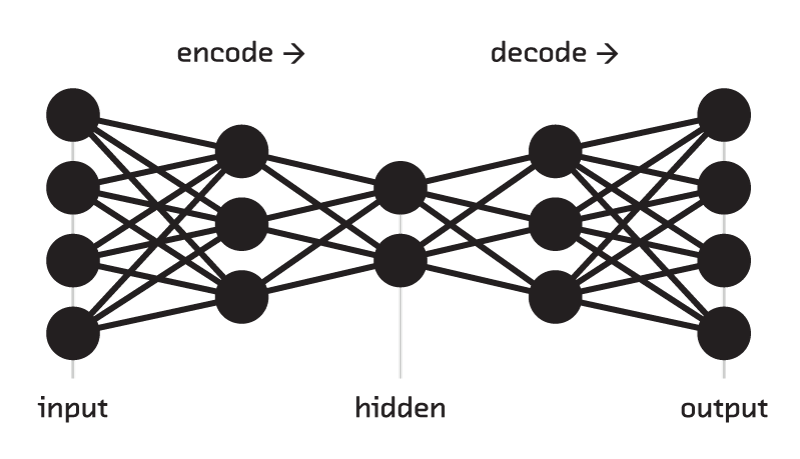
\includegraphics[scale=0.5]{images/basic_autoencoder.png}
\caption{Esquema cl�isco de auto-encoder}
\label{autoencoder_schema}
\label{contexto:figura}
\end{figure}

\par Un auto-encoder esta basado en el paradigma codificador-decodificador \ref{autoencoder_schema}, donde el codificador se encarga de transformar la entrada en, tipicamente, en una repesentaci�n de baja dimensiaonalidad, mientras que el decodificador trata de usar esa salida de baja dimensionalidad para reconstruir la entrada original \cite{AutoEncoderSurvey}. Esta capa intermedia recibe habitualemente el nombre de espacio latente. 
\par La versi�n cl�sica de este modelo estad�stico solo conten�a una capa oculpa, la cual era una representaci�n de baja dimensionalidad de los datos de entrada. En la �ltima d�cada, el auge de las redes neuronales profundas, �mbito m�s conocido por \textit{Deep Learning}, ha provocado el uso de arquitecturas m�s complejas en los autoencoders, con varias capas ocultas tanto en el codificador como en el decodificador. En comparaci�n con los modelos c�sicos de auto-encoders se han mejorado ampliamente los resultados, a�n cuando el n�mero de par�metros a caracterizar es el mismo en ambos sistemas. 
 
 \par Un auto-encoder basado en aprendizaje profundo es capaz de extraer caracter�sticas de manera jerarquica gracias a sus distintas capas ocultas. Existen diferentes aproximaciones entre las que cabe destacar el auto-encoder de filtrado (\textit{Denoising auto-encoder})\cite{AutoEncoderDenoising}, el auto-encoder variacional (\textit{Variational auto-eencoder})\cite{AutoEncoderVariational} o las redes generativas adversarias (del ingl�s \textit{Generative Adversarial Networks}).
 
 \par Los auto-encoders variacionales constituyen una execelente herramienta para la extracci�n de las caracter�sticas principales o de patrones de un espacio muestral, pero tambien pueden ser considerados un modelo generativo\cite{DeepGenerativeModels}, esto es, son capaces de generar datos sint�ticos.  Este modelo es capaz de asociar una distribuci�n gausiana a cada uno de los par�metros fundamentales extra�dos por el propio sistema, esto es, es capaz de caracterizar estad�sticamente a lo que anteriormente denominamos como espacio latente\cite{AutoEncoderVariational}. Esta capacidad es fundamental en cualquier sistema generativo. 
 
 \par Los modelos generativos tienen un amplio rango de aplicacions como son la compresi�n, el filtrado, el aprendizaje no supervisado de caracter�sticas o la s�ntesis de datos.  

\section{Objetivos}

Los principales prop�sitos del presente trabajo son los siguientes:

\begin{itemize}
\item An�lisis e implementaci�n en \textit{Python} de un modelo de autoencoder variacional basado en redes neuronaels densas.
\item An�lisis e implementaci�n de un autoencoder variacional basado en redes neuronales convolucionales.
\item Simular y evaluar la capacidad de s�ntesis de neruoim�genes de cada uno de los dos modelos generativos implentados. Debido a la alta dimensionalidad de las im�genes cerebrales empleadas, se tendr� que realizar la s�ntesis por cada regi�n dado que el an�lisis completo de una imagen necesitar�a unos recursos computacionales y de memoria que no est�n disponibles en los equipos en los que se realizan las pruebas.
\par La necesidad de analizar las r�giones por separado conlleva que se necesiten un conjunto de funcionalidades que permitan manejar este tratamiento de las im�genes. Una de estas funcionalidades es la encargada de reconstruir el cerebro completo a partir de las im�genes 3D de regiones cerabrales en caso de utilizar el modelo convolucional.
\item Ev�luar la capacidad de los dise�os implementados de distinguir entre los suejetos AD de los suejetos NOR, esto es la capacidad de clasificar de forma correcta las distintas neuroim�genes. 
\end{itemize}



 
\chapterend{}
%%%%%%%%%%%%%%%%%%%%%%%%%%%%%%%%%%%%%%%%%%%%%%%%%%%%%%%%%%%%%%%%%%%
%%% Documento LaTeX 																						%%%
%%%%%%%%%%%%%%%%%%%%%%%%%%%%%%%%%%%%%%%%%%%%%%%%%%%%%%%%%%%%%%%%%%%
% T�tulo:		Cap�tulo 2
% Autor:  	Ignacio Moreno Doblas
% Fecha:  	2014-02-01
% Versi�n:	0.5.0
%%%%%%%%%%%%%%%%%%%%%%%%%%%%%%%%%%%%%%%%%%%%%%%%%%%%%%%%%%%%%%%%%%%
\chapterbegin{Contexto}
\label{chp:Utiliz}
%\minitoc

\section{La enfermedad del Alzheimer}
\par En 1906 Alois Alzheimer, describi� las lesiones cerebrales caracter�sticas delvtrastorno que recibi� su nombre: placas seniles y ovillos neurofibrilares. La AD es ahora, 100 a�os despu�s, la forma m�s com�n de demencia en el mundo, estando caracterizada por un espectro de caracter�sticas cl�nicas y fallos neuropat�logicos \cite{AD_historic}.

\par Se han desarrollado numerosos estudios de inverstigaci�n relativos a la naturaleza del AD, no obstante la motivaci�n central ha sido se�alar la AD como una categor�a diferente de la demencia senil \cite{ADhistoric2}, as� como determinar si la AD es la casua principal principal de la demencia en la tercera edad. Hay teor�as que defienden que la AD es una consecuencia natural del envejecimiento, mientras que hay otras que defined lo contrario. 

\begin{figure}[hb]
\centering
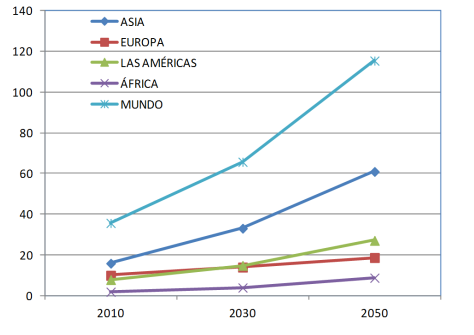
\includegraphics[scale=0.5]{images/evolucion.png}
\caption{Evoluci�n del n�mero de paciente en millones desde 2010 hasta 2050 \cite{Nations}}
\label{AD_evolution}
\label{contexto:figura}
\end{figure}


\par En la actualidad se postula desde la perspectiva de la mitocondria, org�nulo encargado de la respiraci�n celular \cite{mitocondria2} y que toma un papel primordial en el desarrollo de la AD y del propio envejecimiento cerebral. La hip�tesis en casacada de la mitocondria \cite{mitocondriaGeneral} postula que hay mecanismos comunes que conducen al envejecimiento cerebral y a la AD, as� como que la producci�n de placas, ovillos neurofibrilares y la degeneraci�n sin�ptica son consecuencias de la funcionalidad perturbada de la mitocondria. 


\par La AD es uno de los des�rdenos neurodegenerativso m�s serveros y frecuentes en la poblaci�n de la tercera edad teniendo severas repercusiones tanto para la salud como socioecon�micas. El impacto esperado de esta enfermedad se ve incrmentado debido al aumento de la esperanza de vida, se estima que durante los pr�ximos 20 a�os se duplcar� el n�mero de pacientes de dicha enfermedad principalmente en los pa�ses m�s desarrollados.  La figura \ref{AD_evolution}  muestra la evoluci�n del n�mero de pacientes de AD hasta el 2050, en funci�n de los continentes.

\subsection{Fases de la AD}

\subsubsection{Sintomas imperceptibles}
\par  La primera de las se�ales tiene que ver con el descenso de los niveles de la prote�na beta amiloide en el l�quido cefalorraquideo (LCR). Este proceso se puede detectar hasta 25 a�os antes del inicio de la p�rdida de la memoria mediante una resognancia magn�tica. Esta prote�na es la causante de la formaci�n de las placas seniles. Durante esta fase previa a la p�rdida de la memoriase hacen perceptibles las alteraciones en las etructuras tanto en las estructuras cerebrales como en el hipocampo. Es por ello que los s�ntomas se producen varios a�os de que puedan ser percibido por la propia persona o por sus familiares

\subsubsection{Predemencia}
\par Esta fase es usualmente identificada como deterioro cognitivo o conductoal leve. Los primeros sintomas perceptibles son a menudo confundidos con la propia vejecz de la persona. Una evaluaci�n neuropsicol�gica detallada es capaz de determinar evidencias de AD hasta 8 a�os de que se cumplan los crierios de diagn�stico\cite{Predemencia1}.
 
\par La deficiencia m�s relevante es la p�rdida de memoria, ya sea como la incapacidad de adquirir nueva informaci�n o la imposibilidad  de recordad hechos recientes. No obstante pueden aparecer dificultades leves en funciones ejecutivas como la atenci�n o el razonamiento, as� como trastornos en la memoria sem�ntica \cite{Predemencia2}.


\subsubsection{Demencia Inicial}

\par El principal s�ntoma asociado a esta fase inicial es la p�rdida de memoria puntual o incluso una p�rdida de la memoria conocida a corto plazo, la cual supone dificultades para el paciente en la iteracci�n con familiares o amigos. Una peque�a porci�n de los pacientes sufre de dificultades con el lenguaje,  con el reconocimiento de las percepciones o con la ejecuci�n de movimientos. \cite{DemenciaComunicacion} 

\par La capacidad de aprender nuevos conceptos ya sean abstractos o recuerdos reales, esto es, la memoria a corto plazo,  es la que se ve m�s afectada durante esta fase frente a otras capacidades que se ven afectadas en menor medida como es la memoria a largo plazo, la memoria sem�ntica o la memoria impl�cita, la cual hace referencia al conocimiento de como realizar acciones con el propio cuerpo. \cite{DemenciaMemoria}

\subsubsection{Demencia morerada}

\par El s�ntoma diferencial de esta fase con respecto a la anterior son los cambios de conducta inesperada, incluso arranques violentos en personas que nunca han experimentado este comportamiento. Las manifestaciones neuropsiqui�tricas m�s comunes son las distracciones, el desvar�o y los episodios de confusi�n al final del d�a, as� como la irritabilidad y la labilidad emocional, que incluyen llantos o risas inapropiadas. \cite{ADconducta}

\par Los s�ntomas de fases anteriores anteriores se ven acrecentados provocando que el paciente sea incapaz de realizar tareas de cierta complejidad. Los problemas del lenguaje se hacen cada vez m�s evidentes, provocando parafasia. Las capacidades para leer y escribir tambi�n empeoran progresivamente. La memoria impl�citia y la memoria a largo que hasta entonces hab�an estado intactas tambi�n empiezan a verse afectadas. \cite{DemenciaComunicacion}

\subsubsection{Demencia avanzada}

\par Esta fase �ltima de la enfermeda trae el deterioro de la masa muscular del paciente, perdiendose la movilidad, la capacidad de autoalimentarse y en �ltima instancia el encamamiento del paciente. 
\par El lenguaje se vuelve totalmente desorganizado, incluso llegandose a perder completamente \cite{DemenciaComunicacion}. No obstante se conserva la capacidad de detectar y expresas se�ales emocionales. 

\par La AD en s� no produe la muerte del paciente, si no que el fallo de otros sistemas que se ven afectados son los que la provocan. Los pacientes de Alzheimer pueden presentar dificultad para tragar y pueden inhalar los alimentos, lo cual puede originar neumon�a por aspiraci�n. La neumon�a es la causa de la muerte en dos tercios de todas las muertes de pacientes de demencia, seg�n la Sociedad de Alzheimer.

\subsection{S�ntomas}

\par Los s�ntomas asociados en la AD var�a en funci�n de las caracteristicas de cada individuo, por lo que es posible que se presente en diferente grado o incluso orden en funci�n del paciente. Estos s�ntomas se agrupan en tres �mbitos.

\subsubsection{S�ntomas Cognitivos}
\par Se ven afectadas la memoria a corto plazo en fases tempranas de la AD y seguidamente la memoria a largo plazo. La orientaci�n espacial y temporal y la capacidad de ejecuci�n tambi�n se ven afectadas. El s�ntoma principal es la incapacidad gradual de recordad a corto plazo debido a la lesiones que se producen en el hipocampo \cite{hipocampo}.

\subsubsection{S�ntomas Psicopatol�gicos}
\par Se empiezan a presentar cambios conductuales como depresi�n,  ansiedad, agresividad o trastorno del sue�o. Estos cambios en el paciente estan originados por los da�os del l�bulo frontal. 

\subsubsection{S�ntomas funcionales}
\par La interrelaci�n entre los s�ntomas cognitivos, psicol�gicos y conductuales provocan la incapacitaci�n del paciente para realizar las tareas cotidianas habituales as� como la limitaci�n para emprender otras nuevas.

En esta lista se indican algunos s�ntomas cotidianos asociados al AD:

\begin{itemize}
\item Cambios de memoria que dificultan la vida cotidiana.
\item  Dificultad para planificarse y resolver problemas.
\item  Dificultad para resolver tareas en la casa, en el trabajo o en el tiempo libre.
\item  Desorientaci�n de tiempo o lugar.
\item  Dificulta para comprender im�genes visuales y c�mo los objetos se relacionan uno
al otro en el ambiente.
\item  Colocaci�n de objetos fuera de lugar.
\item  Disminuci�n o falta de buen juicio.
\item  Perdida de iniciativa en el trabajo o en actividades sociales.
\item  Cambio en el humor o la personalidad.
\end{itemize}


\subsection{Histopatolog�a}
\begin{figure}[hb]
\centering
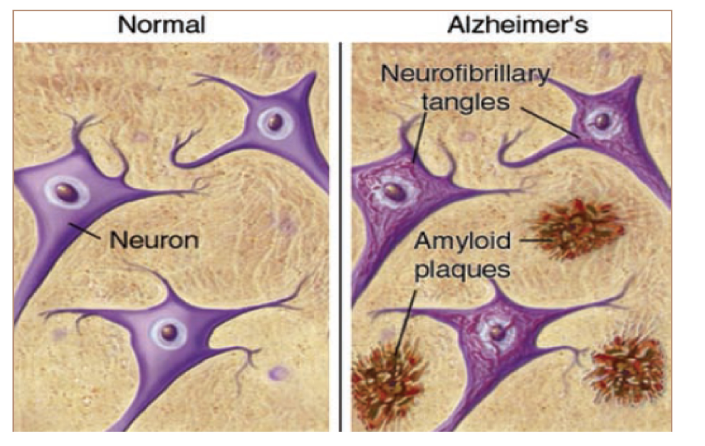
\includegraphics[scale=0.4]{images/ovillos.png}
\caption{Ovillos neurofirilares y placas seniles delos pacientes con AD respecto a los normales. Figura obtenda de \cite{atlasAlzheimer}}
\label{ovillos}
\label{contexto:figura}
\end{figure}



\par Las lesiones neuropatol�gicas comienzan a desarrollarse a�os antes de la completa expresi�n de la demencia cl�nica. Actualmente se desconoce cual es el origen de este proceso de degeneraci�n o porque los procesos normales asociados al envejecimiento se vuelven mucho m�s extremos en pacientes de esta enfermedad. 

\par Desde una perspectiva patol�gica, los dos elementos caracter�stcos de la AD que son las placas neur�ticas, la cual contiene la prote�na beta amiloide ($A \beta$) y los ovillos neurofibrilares sirven como l�nea divisoria entre la AD y otras demencias,
ve�se la Fig. \ref{ovillos}.


\begin{figure}[b]
\centering
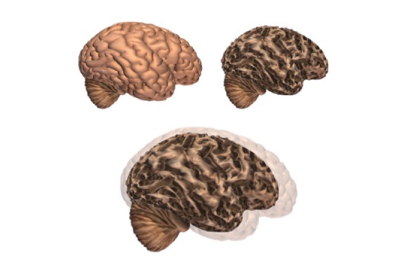
\includegraphics[scale=0.4]{images/imagen2.png}
\caption{Ovillos neurofirilares y placas seniles delos pacientes con AD respecto a los normales. Figura obtenda de \cite{atlasAlzheimer}}
\label{ovillos}
\label{contexto:figura}
\end{figure}
\
\label{sec:TestSuiteCrec}



\par En la AD los ovillos neurofibrilares tienden a ser mas numerosos en las estructuras del l�bulo temporal, incluyendo el hicopocampo. Dentro del hipocampo los ovillos nuerofibrilares tienede a ocupar gran parte del espacio dejado por las neuronas piramidales muertas.  

\par Debido al dep�sito y acumulaci�n de placas seniles y ovillos neurofibrialres se genera estr�s resultante de la inflamaci�n y oxidaci�n que se a�aden a la cadena patol�gica de las consecuencias

\par A medida que aumenta la enfermedad se ve reducido el n�mero de ce?ulas nerviosas y de conexiones entre ellas provocando un deterioro notable del cerebro como se aprecia en la imagen. 

\newpage
\section{Base de datos ADNI}

\par Las im�genes empleadas en este proyecto pertenecen a la iniciativa de neuroimagen de la enfermedad de Alzheimer (ADNI, del ingl�s \textit{Alzheimer Disease Neuroimaging Initiative}). Esta iniciativa fue fundada en 2004 \cite{MainADNI} por un conjunto de instituciones de la salud norteam�ricas en colaboraci�n con diferentes compa�ias farmace�ticas. Una de las instituciones fundadores m�s reconocidas es Instituto Nacional de la Salud (NIH, del ingl�s \textit{National Institute of Health} creado en 1887, siendo actualmente referente en el �mbito de la salud en Estados Unidos. 

\par Esta iniciativa re�ne a las principales instituciones m�dicas tanto en Estados Unidos como en Canada, siendo la organizaci�n que lidera las investigaciones dirigidas al entendimiento de los biomarcadores del cerebro asociados con el funcionamiento cognitivo del mismo. El investigador principal de esta iniciativa es Michael Weiner, profesor de la Universidad de California. 

\par Hasta la fecha se han registrado hasta 1500 personas de entre 50 y 90 a�os en conjunto de los diferentes protocolos de la iniciativa. Se trata de una base de datos longitudinal de sujetos de la tercera edad, o cercanos a ella, que padecen AD o MCI.

\par Los princpales objetivos de la inicitiva ADNI son los siguientes \cite{MainADNI}:
\begin{itemize}
\item El desarrollo de m�todos �ptimos para la estandarizaci�n de la adquisici�n de biomarcadores, especialmente neuroim�genes, tanto MRI como PET , de una manera longitudinal sobre individuos que padecen AD o MCI.  
\item Uso de esto m�todos �ptimizados de adquisici�n de im�gentes longitudinales, tanto estructurales como met�bolicas sobre un amplio conjunto de inviduos sanos,  de sujetos MCI o AD, acompa�ando dichas im�genes de una validaci�n cl�nica del estado real de esos pacientes. 
\item Estudio de aquellos biomarcadores, medidas cognitivas o im�genes neurol�gicas que generan el mayor poder de diagn�stico sobre pacientes MCI y AD.
\item Creaci�n de un respositorio de datos, tanto im�genes como informes cl�nicos, con informaci�n longitudinal de cambios cerebrales, de metabolismo, de funcionamiento o de biomarcadores en los individuoes estudiados.  
\end{itemize}

\subsection{Im�genes m�dicas}
\par Las im�genes neurol�gicas constituyen una herramienta esencial para el estudio y el diagn�stico de las trastornos psiqui�tricos de desarrollo neurol�gico. Estas im�genes permiten elestudio longitudinal de aquellos pacientes que sufren un deterioro congnitivo o funcional, adem�s de permitir realizar una comparaci�n con respecto a lo que se conoce como un desarrollo neurol�gico normal.
\par En el trabajo aqu� realizado nos hemos centrado en las im�genes de resonancia mag�ntica y las im�genes tomogr�ficas por emisi�n de positrones.

\subsubsection{Im�genes MRI}
\par Las im�genes de resonancia magn�tica (MRI, del ingl�s \textit{Magnetic Resonance Image}) son im�genes estructurales obtenidas en base a la aplicaci�n de campos magn�ticos sobre un cuerpo.
\par La t�cnica MRI esta basada en la resonancia magn�tica nuclear (NMR, del ingl�s \textit{Nuclear Magnetic Resonance}). Ciertos n�cleos at�micos son capaces de emitir energ�a a una determinada frecuencia al entrar en contacto con un campo magn�tico externo \cite{MRIOrigin3}. Generalmente, son �tomos de hidr�geno los utilizados para la extracci�n de estas im�genes dado que este tipo de �tomos  existen de manera natural en las personas. Por esta razon, los esc�neres eval�an la localizaci�n de la se�al en el espacio, generando una im�gen en funci�n de la intensidad de la se�al generada. Es posible variar el tipo de se�al generada cambiando el tipo de campo magn�tico empleado.
\begin{figure}[b]
\centering
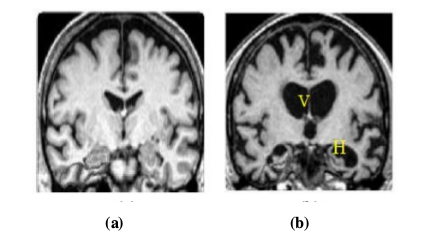
\includegraphics[scale=0.5]{images/mri_brain.png}
\caption{(a) Cerebro con funciones cognitivas normales. (b) Cerebro con funciones cognitivas d}
\label{ovillos}
\label{contexto:figura}
\end{figure}
\
\par Esta t�cnica fu� inventada por Paul C. Lauterbur en Septiembre de 1971 \cite{MRIOrigin}, siendo aplicada por primera vez en el estudio del cerebro por Ian Robert Young y Hugh Clow en 1986 \cite{MRIOrigin2}. Desde entonces es considerada una t�cnica esencial tanto para el estudio del cuerpo humano como parea la investigaci�n biom�dica, covirtiend�se en una herramienta esencial de diagn�stico. 

\par Una de las principales limitaciones de las im�genes MRI es el ruido. El bajo nivel SNR es provocado pr diversos factores, como es la alta emperatura de ruido generada por el esc�ner o el movimiento del cuerpo explorado. Es por ello  que el procesado de filtrado de ruido es uno de los principales �mbitos de investigaci�n en torno as las im�genes MRI \cite{MRINoise}. La tecnolog�a de los escan�res empleados ha evolucionado en aspectos como la resoluci�n espacial o la disminuci�n del tiempo de adquisici�n muestral.

\subsubsection{Im�genes PET}
\par La tomograf�a por emisi�n de positrones (PET, del ingl�s \textit{Positron emission tomography}) es uan t�cnica de estracci�n de im�genes funcionales que permite observar los procesos metab�licos del cuerpo. 
\par Esta modalidad de im�genes neurol�gicas esta basada en la detection de la radioactividad emitida por una peque�o vial inyectado en el paciente. Este vial esta compuesto por radion�clidos, is�topos radioactivos emisores de positrones. Los m�s utilizados en las exploraciones PET son Carbono-11, Nitr�-geno-13, Ox�geno-15, Fluor-18, Cobre-62, Galio-68, Rubidio-82. 
\par Estos is�topos son elegidos principalmente por su corto periodo de vida [13]. Los radion�clidos son incorporados en alg�n compuesto para expandirlo por el organismo, en el caso del Alzheimer lo m�s com�n es la glucosa, a estos compuestos se los conoce como radiof�rmacos. En la actualidad el radiof�rmaco m�s utilizado es el fluorodesoxiglucosa (FDG) donde el fl�or de la mol�cula se convierte en F18. Este radiof�rmaco es el m�s utilizado debido a sus caracter�sticas metab�licas ya que algunos de sus compuestos est�n presentes en el cuerpo humano y tambi�n por su r�pida expulsi�n del organismo sin provocar ning�nefecto secundario. FDG es incorporado principalmente en las c�lulas con elevadas tasas
de glucosa, como por ejemplo el cerebro, donde la fosforilaci�n de la misma impide que sea liberada al metabolismo.

\par En el caso de Alzheimer, debido a su alta tasa de glucosa en la c�lulas cerebrales, la imagen PET muestra una disminuci�n de glucosa en sus fases iniciales lo que nos
permite identificar r�pidamente la enfermedad. Tambi�n se podr� conocer la efectivida de los tratamientos, en cuyo caso se observar� un aumentos del metabolismo cerebral en relaci�n con la situaci�n inicial.






\newpage
\section{Estado del Arte}
\par El presente proyecto tiene como principal objetivo la b�squeda de un modelo estad�stico que nos permita generar neuroim�genes del cerebro, es por ello conveniente exponer algunos m�todos clasicos de modelado generativo as� como otros m�s novedosos en la secci�n que sigue a continuaci�n. 
\par No obstante, dado qu� no existen estudios de la aplicaci�n de la t�cnica usada con un fin generativo sobre neuroim�genes, se expondr� algunos de los trabajos relativos a la detecci�n y el diagn�stico temprano de AD mediante computador con objeto de mostrar el alto �ndice de acierto en el diagn�stico de las t�cnicas actuales.


\subsection{Modelos Generadores}
\par En estad�stica, se define por modelo generador aquel sistema o modelo capaz de generar muestras (u observables) pertenecientes a una determinada clase o tipo respetando la funci�n de distribuci�n conjunta, esto es, una funci�n de distribuci�n multivariada asociada a dicho tipo. 

\subsubsection{Modelos cl�sicos}
 
\par Un modelo generador viene definido por un conjunto de distribuciones de probabilidad las cuales son capaces de aproximar de manera adecuada un conjunto de datos. 
\par Uno de los m�todos tradicionalmente m�s empleados es el \textbf{Modelo de Mezcla de Gausianas}. Se trata de un modelo probabil�stico que asume que todos los observables de un conjunto de datos son generados por un conjunto finito de gausianas. La obtenci�n del modelo se basa en estimadores de maxima verosimilitud.

\begin{figure}[b]
\centering
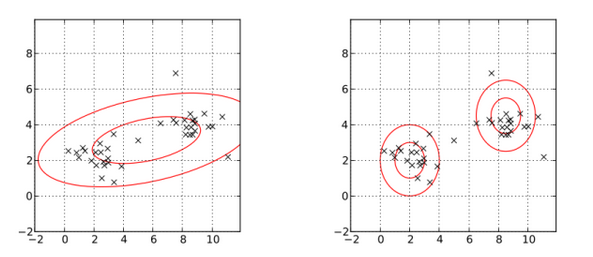
\includegraphics[scale=0.5]{images/captura_GMM.png}
\caption{(Izquierda) Modelo de una �nica Gausiana, (Derecha) Modelo de mezcla de Gausianas}
\label{gmm}
\label{contexto:figura}
\end{figure}

\par EL GMM es una de las t�cnicas m�s usadas para el modelado de datos del mundo de real. Intuitivamente podemos pensar en este m�todo como la mezcla de varias gausianas mono-modales. 

\par Un \textbf{Modelo Oculto de M�rkov} (HMM, del ingl�s \textit{Hidden Markov Model}) es un modelo generador que asume que el proceso o sistema a modelar es un proceso de Markov. El objetivo es determinar los par�metros desconocidos de dicha cadena a partir de los par�metros.  
\par Un HMM  genera de manera explicita la distribuci�n de probabilidad de los estados del proceso evaluado debido a la probabilidad condicional de transici�n entre estados, es por ello que es considerado un modelo generativo. Este tipo de  modelos han sido ampliamente usado �mbitos como el reconocimiento del habla o en teor�a de colas. 


\begin{figure}[t]
\centering
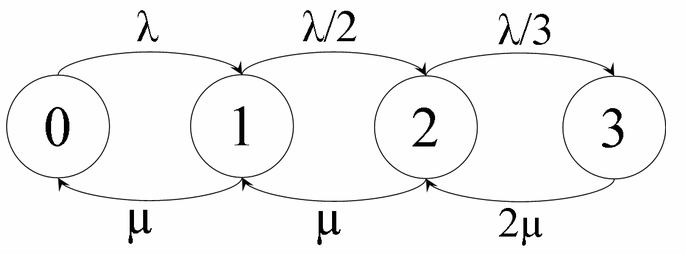
\includegraphics[scale=0.4]{images/markov_chain.png}
\caption{(Izquierda) Modelo de una �nica Gausiana, (Derecha) Modelo de mezcla de Gausianas}
\label{markov}
\label{contexto:figura}
\end{figure}


\subsubsection{La M�quina de Boltzmann}
\par Una M�quina de Boltzman (BM del ingl�s \textit{Boltzmann Machine}) es un tipo de red neuronal estoc�stica. Esta t�cnica puede emplearse para la obtenci�n o aprendizaje de la distribuci�n de probabilidad del conjunto de muestras en cuesti�n. 
\par Dado que  este proceso es costoso, se suele imponer un conjunto de restricciones en la topolog�a de la red neuronal lo cual se conoce como m�quina restrictiva de Bolzman (RBM, del ingles \textit{Restrictive Bolzmann Machine}). \cite{rbm} 
\par Una RBM es un modelo generativo parametrizado que representa una probabilidad de distribuci�n. Dado un conjunto de observaciones, la elaboraci�n de una RBM implica el ajuste de los par�metros con el objetivo de que la distribuci�n de probabilidad asociada a la BM sea lo m�s similar posible a  la distribuci�n real de los datos. 

\par Tras un proceso de aprendizaje exitoso, uno RBM es capaz de extraer la distribuci�n de probabilidad latente u oculta en un conjutno de datos. Esto puede ser empleado como referencia a la comparar con nuevas muestras, lo que se conoce como proceso de clustering clasificatorio,  o puede permitirnos extraer muestras del conjunto muestreando a partir de la distribuci�n aprendida.  

\begin{figure}[t]
\centering
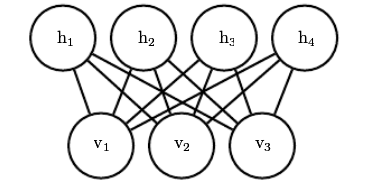
\includegraphics[scale=0.5]{images/RB.png}
\caption{M�delo b�sido de RBM}
\label{rbm}
\label{contexto:figura}
\end{figure} 

\par En la figura \ref{rbm} se puede observar un modelo cl�sico de RBM. Las caracte�sticas principales de este modelo son:
\begin{itemize}
\item Esta constituido por dos partes bien diferenciadas; una capa de unidades ocultas y otra de unidades visibles. A menudo la unidades visibles son referenciadas como estados visibles.
\item No hay conexiones entre unidades de una misma capa.
\item Las unidades ocultas estan probabilisticamente condicionadas a las unidades visibles, aunque son independientes entre s�. 
\item El uso de RBM concatenadas permite la extracci�n de caracter�sticas mas complejas, ver figura \ref{rbms}. En este modelo, el cual es com�nmente denominado \textit{stacked RBMs},  las unidades ocultas(\textit{h}) se convierten en los datos de entradas de las siguientes capas. 
\end{itemize}

\begin{figure}[t]
\centering
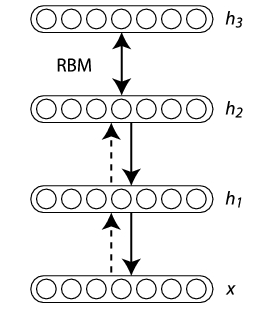
\includegraphics[scale=0.5]{images/rbms.png}
\caption{\textit{Stacked} RBMs}
\label{rbms}
\label{contexto:figura}
\end{figure} 


\par Las RBM son consideradas redes neuronales aplicables para el aprendizaje no supervisado, capaces de caracterizar un espacio muestral. Otra modelo similar es el Autoencoder, t�cnica empleada en este trabajo.  

\subsubsection{Autoencoder}
\par Se conoce como Autoencoer al tipo de red neuronal que tiene como objetivo la caracterizacion de un conjutno de datos con objeto de imitar el dato de entrada a la salida de la red. Esta proceso de imitaci�n esta basado en la extracci�n de caracter�sticas, las cuales son obtenidas en lo que se denomina como capa latente. Esto permite que los autoencoders sean un m�todo de reducci�n de dimensionalidad altamente empleado. 
\par En el siguiente cap�tulo se profundizar� en las expresiones matem�ticas por lo que durante este �nicamente se dar� una visi�n general del modelo.

\begin{figure}[h]
\centering
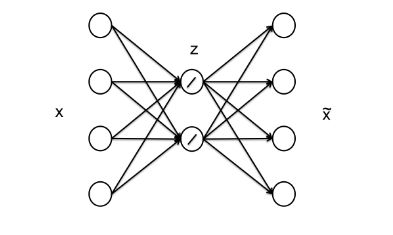
\includegraphics[scale=0.5]{images/linear_autoencoder.png}
\caption{Autoencoder Lineal}
\label{autoencoder2}
\label{contexto:figura}
\end{figure}

\par En la figura \ref{autoencoder2} se puede observar un modelo de Autoencoder b�sico denominado Autoencoder Lineal. Las caracter�sticas principales son:
\begin{itemize}
\item Codificaci�n: $\boldsymbol{Z} = \boldsymbol{F(X)}$. 
\textbf{F(X)} es la funci�n de codificaci�n basada en los productos de los datos de entrada y unos pesos, obtenidos durante el entrenamiento, aplicandose una funci�n de activaci�n, tipicamente la funci�n sigmoide. 

\item Decodificaci�n. $\hat{\boldsymbol{X}} = \boldsymbol{G(Z)}$. \textbf{G(X)} realiza el proceso inverso, tomando como entrada el vector de valores del expacio latente \textbf{Z}. 
\end{itemize}

\par Si el espacio latente \textbf{Z} tiene una dimensionalidad menor que el espacio \textbf{X}, entonces la funci�n \textbf{F} tiene capacidad de compresi�n sobre las muestras de entrada \textit{x}. Es por ello que un vector latente \textit{z}, obtenido a partir de un vector de entrada \textit{x}, puede considerarse una representaci�n de dimensionalidad reducidad de \textit{x}. 

\par Es interesante mencionar que en este caso tanto \textbf{F(X)} como \textbf{(G(Z)} son funciones deterministas, a diferencia de las empleadas en  una RBM, donde son funciones probabilisticas. 
\par Las principales aplicaciones del Autoencoder son la extracci�n de caracter�sticas de las muestras a partir de la capa latente \textbf{Z} y la posibilidad de generaci�n de nuevas muestras con unas caracter�sticas similares a las utilizadas durante el proceso de caracterizaci�n del modelo. Esta capacidad de generaci�n se basa en modificar los c�digos latentes \textit{z} de las muestras \textit{x}. 

\par No obstante, una de las principales limitaciones asociados a este modelo lineal de autoencoder es la posibilidad de que la funci�n codificadora y decodificadora �nicamente aprendan una funci�n identidad de la muestra de entrada, lo cual imposibilita tanto el proceso de reduccion de dimensionalidad sobre  muestras no observadas durante el proceso de entrenamiente como el proceso de generaci�n de nuevas muestras.

\par El Autoencoder de filtrado (denominado \textbf{\textit{denoising Autoencoder}} en ingl�s) tiene como objetivo evitar dicho problema \cite{denoising_autoencoder}. Para ello a todas las muestras de entrada \textit{x} se les aplica un ruido no determinista con objeto de forzar que la capa latente tenga que aprender caracter�sticas robustas que extraigan pasnciones identidad de las muestras. 

\par Un Autoencoder de filtrado realiza tres acciones principales:
\begin{itemize}
\item Mezclado de ruido. La muestra de entrada \textit{x} es mezclada con un ruido aleatorio. 
\item Codificaci�n. El c�digo latente generado \textit{z} debe preservar la informaci�n primaria de la muestra previa al mezclado del ruido.
\item Decodificaci�n. La muestra de salida $\hat{x}$ ha de ser lo m�s parecida posible a la muestra de entrada \textit{x}.  
\end{itemize}

\par En el trabajo realizado por Pascal Vincent y Hugo Laroche en 2008 \cite{denoising_autoencoder2}, el ruido es introducido en las muestras mediante un proceso estoc�stico asignando cero a algunos de los valores de las muestras. En este caso el Autoencoder de filtrado est� intentando caracterizar o "predecir" los valores eliminados a partir de los valores presentes de las muestras. 

\par Gracias al reciente de las redes profundas, se han propuesto modelos de autoencoders cada vez m�s complejos con varias capas intermedias, lo cual permite extraer caracter�sticas m�s complejas. El \textbf{Autoencoder Variacional} (\textit{VAE} del ingl�s \textit{Variational Autoencoder}) se ha convertido en uno de los m�todos mas populares para el aprendizaje no supervisado de distribuciones complicadas. 

\par El VAE, a diferencia de los modelos de autoencoders cl�sicos, busca la caracterizaci�n del espacio muestral de entrada no mediante una funci�n determinista sino con una funci�n de probabilidad, realizando una serie de restricciones sobre la funci�n de distribuci�n de los valores del espacion latente. Los conceptos matem�ticos en profundidad relativos a este algoritmo ser�n explicado en el pr�ximo cap�tulo debido a que es la principal herramienta en este trabajo. 

\subsubsection{Red Generativa Adversaria}
\par Otro modelo novedoso, impulsado por el desarrollo de las redes neuronales profundas, es la Red Generativa Adversaria\cite{gan}. Este modelo tiene una alta capacidad de caracterizaci�n, siendo capaz de generar images realmente realistas. \cite{gan_example}.

\begin{figure}[h]
\centering
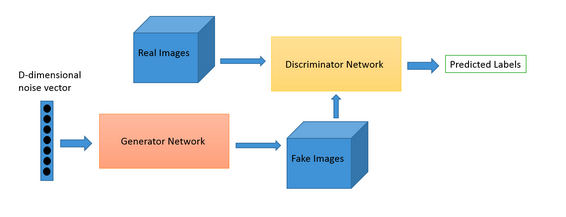
\includegraphics[scale=0.6]{images/gan.png}
\caption{Esquema de una Red Generativa Adversaria}
\label{autoencoder2}
\label{contexto:figura}
\end{figure}

\par En este tipo de modelos tenemos dos redes bien diferenciadas la red generadora y la red discriminadora. Normalmente, la red generadora es la encargada de generar las muestras a partir del espacio latente, mientras que la red discriminadora ha de comparar la muestras generadas con las originales del espacio muestral con objeto de determinar si verdaderamente se pueden considerar muestras artificiales de dicho espacio. 
\par El proceso de entrenamiento de la red generativa tiene como objetivo generar muestras que sean lo m�s parecidas a las originales, y por lo tanto, que no puedan ser detectadas por el discriminador. Mientras que el objetivo del entrenamiento de la red discriminativa es justo el contrario, esto es, ser lo mas estricta posible. 
\par Es por ello que el entrenamiento de este sistema es realmente complejo, considerandose m�s complicado de conseguir unos valores de entrenamiento �ptimos que con respecto al VAE.


\subsubsection{Trabajos Previos}

\par En la b�squeda de estudios similares al aqu� desarrollado nos encontramos con el trabajo desarrollado por Eunbyung Park de la universidad de Carolina del Norte, Estados Unidos. Este trabajo parte con el objetivo de la extracci�n de caracter�sticas �tiles de im�genes MRI tanto para el diagn�stico del AD como para su uso generativo \cite{vae_2d}. 
\par En dicho trabajo se usa un autoencoder variacional convoluciaonal 2d, lo cual difiere de los empleados en nuestro trabajo que, como se explcar� m�s adelante, son convolucionales 3D o totalmente densos. 
\par Se expone como dicho modelo es capaz de caracterizar componentes estrucuturales de las im�genes, permitiendo diferneciar la informaci�n generad en un espacio 2d, aplicando reducci�n de dimensionalidad mediante T-SNE. No obstante, se menciona como las im�genes regeneradas son algo borrosa, algo caracter�stico del VAE.  



\begin{figure}[h]
\centering
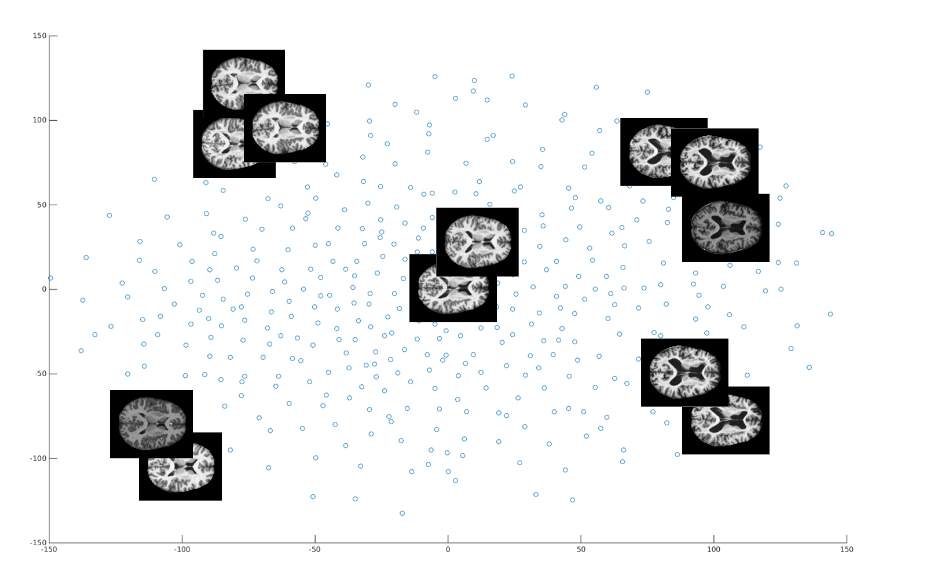
\includegraphics[scale=0.4]{images/tsne_generative.png}
\caption{Visualizaci�n del espacio de dimensionalidad reducida conseguido en el trabajo \cite{vae_2d}. Las im�genes superpuestas corresponden a las imagenes reales, no a las generadas}
\label{tsne}
\label{contexto:figura}
\end{figure}

\par Ea figura \ref{tsne} se aprecia como es posible la diferenciaci�n por caracter�sticas principales de las im�genes MRI en un espacion de dos dimensiones. 

\newpage
\subsection{Diagn�stico Asistido por Computador de AD}
\par Aunque el objetivo final del trabajo es generar im�genes �tiles para el diagn�stico y estudio del AD debido a los escasos trabajos que apliquen el VAE a este fin, se cree conveniente la exposici�n de las siguientes t�cnicas de diagn�stico, ya que es necesario para comprender la utilidad y el estado actual de las diferentes herramientas del �mbito tratado. 
\par Durante la �ltima d�cada se han desarrollado todo tipo de aproximaciones para el diagn�stico de AD asistido por computador. Este gran desarrollo es debido, en parte, a asociacones de gran calado como ADNI. 
\par En este tipo de t�cnicas CAD, normalmente nos encontramos con dos fases bien diferenciadas, una es la extracci�n de caracter�sticas mientras que la siguiente es la clasificaci�n realizada sobre dichas caracter�sticas.


\begin{figure}[h]
\centering
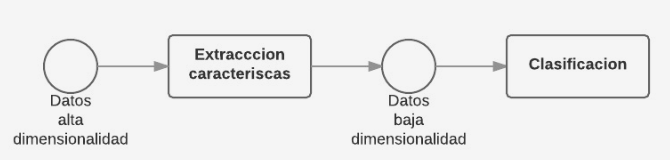
\includegraphics[scale=0.6]{images/basic.png}
\caption{Esquema cl�sico b�sico de un sistema de diagn�stico de AD asistido por computador}
\label{basic_cad}
\label{contexto:figura}
\end{figure}

\subsubsection{M�todos Clasicos}

\par Algunas t�cnicas cl�sicas de extracci�n de caracter�sticas son las siguientes \cite{mri_survey}: 

\begin{itemize}
\item An�lisis de componenets independientes (ICA, del ingl�s \textit{Indepenedent Component Analysis}). Esta t�cnica de transformaci�n de par�metros permita capturar informaci�n de un orden alto de dimensionalidad y transformarlo a un orden menor, utilizando componentes vectoriles estad�sticiamente diferentes. \cite{ica}
\item An�lisis de Componentes Principales (PCA, del ingl�s \textit{Principal Component Analysis}). Esta t�cnica es usada cuando el objetivo es reducir el n�mero de caracter�sticas y convertirlas a un espacio de alta varianza y menor dimensionalidad \cite{pca}. 

\item \textit{Wavelets}. Se trata de un conjunto de funciones matem�ticas encargadas de descomponer los datos en funci�n de la frecuncia. La Transformada de Fourier solo genera informaci�n  frecuencial relativa al contenido, es por ello, que la Transformada \textit{Wavelet} es una mejor herramienta para el estudio de las im�genes. \cite{wavelet}

\item Matriz de co-ocurrencieas de niveles de gris (\textbf{GLCM} del ingl�s \textit{Gray Level Co-Occurence Matrix}). Esta t�cnica est� basada en la estracci�n de caracter�sticas estad�sticas de la imagen. La matriz caracteriza la distribuci�n de los niveles de gris de una imagen o de una region.

\end{itemize}  


\par Algunos de los m�todos que se expondr�n a continuaci�n son utilizados para la clasificaci�n de los vectores de datos generados por los m�todos de extracci�n de caracter�sticas.

\begin{itemize}
\item Clasificador KNN (del ingl�s \textit{K-Nearest neighbor}). Este m�todo de clasificaci�n es uno de los m�s usados historicamente \cite{knn}. Este clasificador se basa en la evaluaci�n de la distancia de una muestra en cuesti�n $x_i$ con respecto al conjunto de clases o instancias posibles $M$, previamente predefinidas durante el entrenamiento. Se considerar� que la muestra $x_i$ pertenecer� a la clase $m$ con respecto a la cual la distancia sea la m�nima.  

\item Clasificador de Bayes (\textit{Na�ve bayes Classifier}). Se trata de un clasificador basado en el teorema de Bayes. En este clasificador se considera que todas las caracter�sticas contribuyen de manera independiente a la probabilidad de pertener a una clase u otra, sin tener en cuenta la presencia del resto de variables. 

\item  Maquina de Vectores de Soporte (SVM del ingl�s \textit{Support Vector Machine}). Este m�todo de clasificaci�n es uno de los mejores algoritmos de aprendizaje supervisado, siendo dise�ado originariamente para la clasificaci�n binaria. 
\par Este ser� el m�todo usado en este trabajo  para la evaluaci�n de las caracter�sticas extra�das por el sistema usado, en nuestro caso es un Autoencoder Variacional, siendo las caracter�sticas los valores de la capa latente. Algunos detalles de este algoritmo ser�n expuestos en siguientes cap�tulos.
\end{itemize}  

\subsection{M�todos de Aprendizaje Profundo}

\par Aunque las t�cnicas anteriormente expuestas constituyen los m�todos cl�sicos relativos a las herramientas CAD, son los m�todos basados en aprendizaje profundo (\textit{deep learning}) los que han conseguido los mejores resultados de clasificaci�n \cite{deep_learning}. 
\par En estas t�cnicas de aprendizaje se han conseguido m�s de un 95\% de precisi�n en el diagn�stico del Alzheimer \cite{deep_learning_2}\cite{deep_learning_3}. 
\par Estas t�cnicas hacen uso de redes neuronales capaces de extraer caracter�sticas complejas de las im�genes. En algunos casos, se emplean un primer tipo de red, como por ejemplo de un Autoencoder, como m�todo de extracci�n de caracter�sticas y seguidamente un m�todo de clasificaci�n ya se cl�sico o basado tambi�n en aprendidaje profundo. 
\par Generalmente se usa un tipo de red neuronal denominadas redes neuronales convolucionales (CNN del ingl�s \textit{Convolutional Neural Networks}), ideales para la extracci�n de informaci�n de las im�genes. Este tipo de redes estan basadas en el comportamiento de la vista humana, ya que son capacades de extraer informaci�n espacial de los datos, lo cual es ideal para las im�genes 

\par En el trabajo realizado por Ehsan Hossini-Asl y Robert Keynton  se consiguen resultados de exactitud de 97.6\% en la diferenciaci�n de pacientes AD de los NC, mientras que consigue hasta un 90\% en la diferenciaci�n de los MCI de los AD \cite{cnn_ad_1}. Este trabajo emplea un modelo  convolucional 3D, capaz de aprender caracter�sticas genericas empleando para ello un Autoencoder, el cual es entrenado para capturar las variaciones estructurales en las im�genes MRI. 
\par El planteamiento realizado en este trabajo es diferente al nuestro dado que se emplea un tipo de autoencoder en el que se capturan variables locales debido al uso de conexi�n mediante nodos locales en lugar de conexi�n global que es nuestro caso. A priori, el empleo de conexiones no globales puede dificultar la extracci�n de caracter�sticas, pero permite reducir de forma notable el tiempo necesario para el entrenamiento del sistema. Por otro lado, en nuestro trabajo se eval�an im�genes seccionadas por regiones cerebrales, en lugar de emplear im�genes completas.  

\begin{figure}[h]
\centering
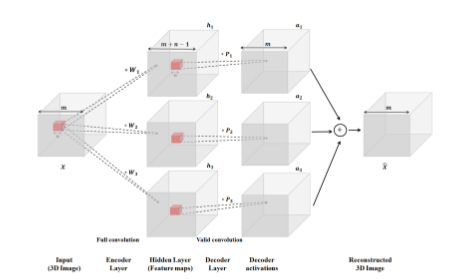
\includegraphics[scale=0.8]{images/autoencoder_2.png}
\caption{Diagrama del Autoencoder Convolucional 3D empleado en el trabajo \cite{cnn_ad_1} para la extracci�n de caracter�sticas}
\label{basic_cad}
\label{contexto:figura}
\end{figure}

\par Como m�todo de clasificaci�n se emple� una red neuronal densa, esto es, totalmente conectada entre las unidades de capas adyacentes, la cual  recib�a los datos generados por el Autoencoder. 

\begin{figure}[ht]
\centering
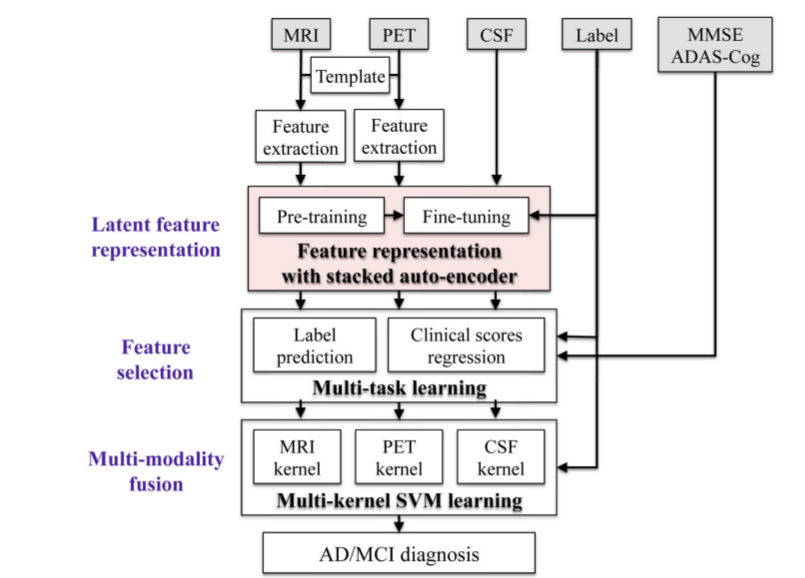
\includegraphics[scale=0.45]{images/autoencoder_3.png}
\caption{Diagrama general del m�todo desarrollado en el trabajo \cite{cnn_ad_2}}
\label{SA_2}
\label{contexto:figura}
\end{figure}

\par Uno de los primeros estudios enfocados a la aplicaci�n de aprendizaje profundo para el diagn�stido de AD fue el desarrollado por Heung-Il y Dinggang Shen en 2013 \cite{cnn_ad_2}. Es interesante notar como un Autoencoder es usado como m�todo de extracci�n de caracter�sticas. El modelo propuesto en este estudio es el de la imagen \ref{SA_2}.
\par La principal innovaci�n de este m�todo es la capacidad de extracci�n de correlaciones no lineales entre los datos gracias al uso de un autoencoder, lo cual teoricamente permite la extracci�n de mejores caracter�sticas globales.  
\par Se trata de un modelo de diagn�stico multimodal ya que emplea diferentes tipos de neuroim�genes como son MRI, PET y CSF. Se emplea un Autoencoder en cascada, que permite la extracci�n de caracter�stcas, pero a diferencia del modelo Variacional, usado en este trabajo, este modelo de Autoencoder emplea una funci�n determinista en lugar de probabil�stica. Como herramienta de clasificaci�n se emplea un SVM multikernel, aplicado cada kernel a las diferentes fuentes de datos. 
\par Los resultados indicados son de un 95\% de exactitud en la diferenciaci�n  AD sobre NC. 
\newpage
\section{Entorno de desarrollo}

\par Los diferentes elemtnos software generados en este proyecto han sido desarrollados sobre Python. Este lenguaje de programaci�n cuenta con una comunidad cient�fica en auge. Los principales motivos por lo que se ha seleccionado son: 
\begin{itemize}
\item Se trata de un lenguaje de c�digo libre, lo cual evita cualquier tipo de coste asociado a la licencia de lenguaje. 
\item Cuenta con reconocidas librer�as de m�todos n�mericos y estad�sticos que agilizan el desarrollo de los modelos. Algunas de estas librer�as son \textit{SciPy, Numpy o Sklearn}. \textit{Numpy} es una librer�a que trabaja con vectores, lo cual resulta ideal para cien�ficos provenientes del entorno Matlab.
\item Debido a su amplia comunidad hay una gran cantidad de c�digo en repositorios p�blicos los cuales son �tiles como referencia. 
\end{itemize}

\par Para el desarrollo de los algoritmos basados en aprendizaje profundo hemos hecho uso de \textit{Tensorflow} \cite{tensorflow}. Esta biblioteca desarrollado por \textit{Google} constituye una interfaz para el desarrollo de algoritmos de aprendizaje que facilita la implementaci�n de dichos algoritmos. 

\par El c�digo de esta librer�a fu� hecho p�blico por \textit{Google} el 9 de Noviembre de 2015. \textit{Tensorflow} fu� originalmente desarrollado por el equipo \textit{Google Brain} desde 2011, denomin�ndose \textit{DisBelief}.

\par Basado en la uni�n de grafos de las diferentes unidades del algoritmo implementado, esta librer�a esta principalmente orientada al desarrollo de redes neuronales, proveyendo m�todos para generar redes neuronales densas y convolucionales. 
\par Otro punto que fomenta el uso \textit{Tensorflow} es la posibilidad de ejecutar los algoritmos sobre tarjetas gr�ficas (GPU, del ingles, \textit{Graphical Processing Unit}) en lugar de sobre el procesador central (CPU, del ingles \textit{Central Processing Unite}).

































\chapterend{}
%%%%%%%%%%%%%%%%%%%%%%%%%%%%%%%%%%%%%%%%%%%%%%%%%%%%%%%%%%%%%%%%%%%
%%% Documento LaTeX 																						%%%
%%%%%%%%%%%%%%%%%%%%%%%%%%%%%%%%%%%%%%%%%%%%%%%%%%%%%%%%%%%%%%%%%%%
% T�tulo:		Cap�tulo 2
% Autor:  	Ignacio Moreno Doblas
% Fecha:  	2014-02-01
% Versi�n:	0.5.0
%%%%%%%%%%%%%%%%%%%%%%%%%%%%%%%%%%%%%%%%%%%%%%%%%%%%%%%%%%%%%%%%%%%
\chapterbegin{Fundamentos Te�ricos}
\label{chp:Utiliz}
%\minitoc

\par El trabajo realizado en este proyecto es englobado dentro de la tem�tica denomiada visi�n por computador, dado que los m�todos empleados se basan en la detecci�n de patr�nes sobre las im�genes dadas, en nuestro caso neuroim�genes. 

\par En el �mbito de la visi�n por computador cada imagen en s� misma es una muestra de miles dimensiones, cada uno de los pixeles. Un modelo generativo trata de capturar la relaci�n entre las multiples dimensiones de los datos. En nuestro caso el modelo empleado para capturar dichas relaciones es el Autoencoder Variacional.

\par Es por ello que este cap�tulo se centrar� en la exposici�n de este m�todo en primer lugar. Dado el VAE esta fundamentado en el aprendizaje profundo, se dedicar� la siguiente secci�n a las redes neuronales, haciendo especial hincapie a aquellas empleadas en este trabajo. Finalmente se expondr�n brevemente los m�todos estad�sticos usados de manera auxiliar a lo largo de este proyecto.  

\section{Autoencoder Variacional}

\par Este apartado est� dedicado a la exposici�n del  Autoencoder Variacional desde una perspectiva meramente te�rica  con objeto de mostrar los fundamentos y, en �ltima instancia, la capacidad de convergencia del m�todo, basada en una funci�n objetivo sobre la cual se puede aplicar descenso en gradiente estoc�stico. 

\subsection{Modelo de Variables Latentes}

\par

\begin{figure}[htp]
\centering
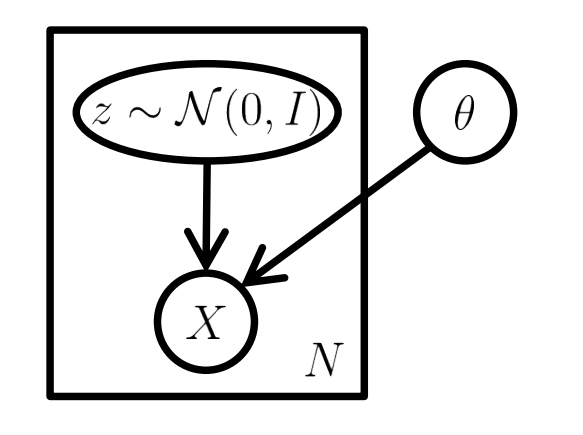
\includegraphics[scale=0.25]{images/ModeloVariablesLatentes.png}
\caption{Modelo gr�fico de variables latentes para el modelo generativo del VAE. $Z$ es el espacio de variables lo m�s similar posible a un distribuci�n normal $(N(0,I))$. El elemento $\theta$ es el conjunto de par�metros que aplicados de manera funcional sobre las variables latentes son capaces de generar el conjunto muestral $X$ }
\label{latentes_variables}
\end{figure}

\par A lo largo del entrenamiento o la caracterizaci�n de un modelo generativo, la parte mas complicada es la extracci�n de las dependencias entre las m�ltiples dimensiones. Son estas relaciones multidimensionales las que permiten generar muestras artificiales pertenecientes a clases distintas. Se denomina variable latente, a las unidades del modelo generativo capaces de discernir entre las distintas clases, esto es, capacitan al modelo para generar elementos diferenciados.



\par Un modelo generativo es representativo de un espacio muestral $(X)$ si para cada una de las muestras de dicho espacio $(x)$ hay al menos alguna configuraci�n de las variables latentes $(z)$ que genera un variable $(\hat{x})$ muy similar a la original. Formalmente, dada una funci�n  $f(z, \theta)$ parametrizada por un vector $\theta$ en un espacio $\Theta$ tal que:
\begin{center}
\begin{equation} \label{eq:space}
f : 	Z \times \Theta  \rightarrow  X  
\end{equation}
\end{center}

\subsection{Modelo Probabil�stico}
\par El objetivo es maximizar la probabilidad de cada $x$ de el espacio muestral de acuerdo con:
\begin{center}
\begin{equation} \label{eq:int_1}
P(X)  = \int_{}^{}P(X|z;\theta) 
\end{equation}
\end{center}
\par En la ecuaci�n \ref{eq:int_1}, $f(z;\theta)$ es reemplazada por la distribuci�n $P(X| z;\theta)$, la cual nos permite hacer expl�cita la dependencia de $X$ sobre $z$, debido a la probabilidad condicionada. 
La idea de detr�s de dicha expresi�n es principio de m�xima verosimilitud (ML, del ingl�s \textit{Maximum Likehood}), el cual indica que si el modelo es capaz de generar muestras del espacio $X$, entonces ser� probable que le modelo generativo construya muestras similares.

\par En el VAE, la funci�n de probabilidad $P(X|z;\theta)$ es las siguiente:

\begin{center}
\begin{equation} \label{eq:p_x_gausiana}
P(X|z; \theta)  = N(X| f(z;\theta), \sigma^{2}*I) 
\end{equation}
\end{center}

\par El uso de una distribuci�n gausiana nos permite emplear descenso en gradiente durante la optimizaci�n, con objeto de caracterizar el modelo. Esta caracterizaci�n permite incrementar $P(X)$, entendidada como la probabilidad global de generar alg�n tipo de muestra de dicho espacio. Esto no ser�a posible si esta funci�n de probabilidad fuera una delta de Dirac. Es importante notar que es fundamental disponener de una funci�n $P(X|z)$ que sea computable y continua sobre $\theta$.

\par Te�ricamente, para la mayor�a de los valores $z$, $P(X|z)$ ser� aproximadaente cero, y por lo tanto su contribuci�npara la estimaci�n de $P(X)$ ser� pr�cticamente nula.

\subsection{Funci�n Objetivo}

\par La principal idea en la que se fundamenta el VAE es en muestrear los valores de $z$ a partir de $X$, esto es, necesitamos una nueva funci�n $Q(z|X)$ que nos permita generar el conjunto de valores del espacio $Z$ a paritr de $X$. Esto nos reduce el espacio de $Z$ ya que, te�ricamente, este se ver� limitado en $Q(z|X)$. En �ltima instacia, esto nos permitir� estimar  $E[P(X|z)]$, siendo esta el valor esperado de la distribuci�n de probabilidad de los valores de X generados. 
\par La relacion entre $E(P(X|z))$ y $P(X)$ es uno de los fundamentos de los m�todos variacionales Bayesianos. Comencemos con la definici�n de la divergencia de KUllback-Leibler (\textit{KL}  o \textit{D}) entre una distribuci�n $P(z|X)$ y $Q(z)$:


\begin{center}
\begin{equation} \label{eq:KL_1}
D[Q(z)||P(z|X)] = E[log(Q(x)) - log(P(z|X))] 
\end{equation}
\end{center}

\par La expresi�n anterior, ecuaci�n  \ref{eq:KL_1}, es una medida no sim�trica de la similitud o diferencia entre las dos funciones de probabilidad $P(X|z) y Q(z)$. Dicha expresi�n mide diferencia (o el extra de informaci�n) entre un co�digo $P(x)$ y uno $Q(z)$. Aplicando la regla de Bayes sobre la expresi�n anterior conseguimos dejarlo en funci�n de $P(X)$ y $P(X|z)$:

\begin{center}
\begin{equation} \label{eq:KL_2}
D[Q(z)||P(z|X)] = E_{z}[log(Q(x)) - log(P(X|z)) - log(P(z)) + log(p(X))]  
\end{equation}
\end{center}

\par Ordenando la expresi�n anterior, y teniendo en cuenta que $log(p(X))$ no depende de $z$ por lo que puede salir del valor esperado:

\begin{center}
\begin{equation} \label{eq:KL_3}
log(p(X))- D[Q(z)||P(z|X)]  = E_{z}[log(P(X|z)]) - D[Q(z)||P(z)].  
\end{equation}
\end{center}

\par Llegados a este punto es importante notar que el espacio $X$ es fijo y por lo tanto tambi�n lo  es su funci�n de probabilidad $P(X)$. No obstante $Q(z)$ puede ser cualquier distribuci�n, siempre que nos permita generar $Z$ a partir de $X$.
\par Dado que en nuestro caso estamos intersados en inferir $P(X)$, es necesario generar una funci�n $Q$ dependiente sobre $X$ que permita que la divergencia $D[Q(z)||P(z|X)]$ sea peque�a, esto es, haya la menor perdida de informaci�n entre ambas distribuciones.

 \begin{center}
\begin{equation} \label{eq:KL_4}
log(p(X))- D[Q(z|X)||P(z|X)]  = E_{z}[log(P(X|z)]) - D[Q(z|X)||P(z)].  
\end{equation}
\end{center}

\par La expresi�n anterior, ecuaci�n \ref{eq:KL_4}, es la principal del VAE, por lo que es necesario examinarla detenidamente. Analizando cada t�rmino por separado:
\begin{itemize}
\item La expresi�n de la izquierda representa la cantidad que se prentende maximizar: $log(P(x))$, mas un t�rmino de error reperesentado por D[Q(z)||P(z|X)] que es la capacidad de generar $z$ a partir de $X$. Este t�rmino de error ser� disminuido si $Q$ es de alta capacidad. 
\par Se trata de maximizar $log(P(X))$ mientras simultaneamente $D[Q(z|X)||P(z)]$ se minimiza . El t�rmino de probabilidad $P(z|X)$ no es computable anal�ticamente, describe la distribuci�n de valores de $z$ que son capacades de generar $X$.
\item La expresi�n de la derecha es lo que se pretende optimar mediante el descenso en gradiente, dada una correcta seleccion de $Q(x)$.
\par Este segundo t�rmino fuerza la similitud entre $(Q(z|X))$ y$ P(X|z)$. Asumiendo que el t�rmino $Q(z|X)$ es de alta capacidad, tendr�mos que el t�rmino de divergencia KL ser� cercano a cero. En �ltima instancia, conseguiremos manejar de forma ana?itica $P(z|X)$ gracias a su similitud con $Q(z|X)$ 
\end{itemize}

\subsection{Optimizaci�n de la funci�n objetivo}

\par Con objeto de poder realizar el descenso en gradiente sobre la expresi�n de la derecha de la ecuaci�n \ref{eq:KL_4}, necesitamos definir de manera m�s exacta la forma de $Q(z|X)$. La elecci�n habiutual es la siguiente:

 \begin{center}
\begin{equation} \label{eq:OFU_1}
Q(z|X)  = N(z|\mu(X;\vartheta), \Sigma(X; \vartheta))  
\end{equation}
\end{center}

donde $\mu$ y $\Sigma$ son funciones determistas con una serie de par�metros $\vartheta$ (en las siguientes expresiones se omitir� $\vartheta$). Normalmente tanto $\mu$ como $\Sigma$ son implementados mediante redes neuronales y $\Sigma$ esta limitada a un funci�n diagonal, que permite facilitar los c�lculos.

\par El segundo t�rmino de la expersion \ref{eq:KL_4}, $D[Q(z|X)||P(z)]$, al ser una divergencia KL entre dos funciones de gausianas multivaradas queda definda por:


 \begin{align*}
 \begin{split}
D(N(\mu_{0}(X), \Sigma_{0}(X)|| N(\mu_{1}(X), \Sigma_{1}(X)))  = \\
\frac{1}{2}\left(tr(\Sigma_{1}^{-1}\Sigma_{0}) + (\mu_{1} - \mu_{0})^{T} \Sigma_{1}^{-1}(\mu_{1} - \mu_{0}) - k + log (\frac{det\Sigma_{1}}{det\Sigma_{0}})  \right)
\end{split} 
 \end{align*}  \label{eq:OFU_2}
 
donde $k$ es la dimensionalidad de la distribuci�n, la expresi�n queda de la siguiente manera:

 \begin{align}
 \begin{split}
D[N(\mu(X), \Sigma(X)) || N(0, I))] = \\
\frac{1}{2} \left( tr(\Sigma(X)) + (\mu(X))^{T}(\mu(X) - k -log(det(\Sigma(X)))) \right)
\end{split} 
 \end{align}  \label{eq:OFU_3}

\par El primer t�rmino de la expresion \ref{eq:KL_4}, $E_{z}[log(P(X|z))]$, es algo m�s complicado de determinar, aunque a priori se podr�a estimar usando un n�mero suficentes de $z$ y aplicando al funci�n $f$ asociada a $P(X|z)$, aunque esto ser�a tremendamente costoso computacionalmente. 
\par En  su lugar, se aplica un procedimiento denomidado Descenso en Gradiente Estoc�stico (SGD, del ingl�s \textit{Stochastic Gradient Descent}), que se basa en tomar �micamente un valor de $z$ aplicarlo sobre $P(X|z)$, por lo que se obtendr�a una aproximaci�n de $E_{z}[log(P(X|z))]$. Durante este proceso, estamos tomando como referencia cada una de las muestras $X$ de un conjunto de datos $D$ a la hora de estimar el error. Teniendo en cuento esto, la ecuaci�n completa que se pretnede optimizar es:

 \begin{align}
 \begin{split}
E_{X}[log(P(X)) - D[Q(z|X) || P(z| X)]] = \\
E_{X}[E_{z}[log(P(X|z))] - D[Q(z|X) || P(z)]]
\end{split} 
 \end{align}  \label{eq:OFU_4}

\par Tomando el gradiente de la expresi�n anterior, reducimos la expresi�n a los valores internos de las esperanzas. Adem�s, podemos tomar un �nico valor de $X$ y un �nico valor de $z$ de la distribuci�n $Q(z|X)$, lo que no nos permite hacer computable el gradiente de la siguiente forma: 

 \begin{center}
\begin{equation} \label{eq:OFU_5}
log(P(X|z)) - D[Q(z|X) || P(z)]. 
\end{equation}
\end{center}

\par No obstante hay un problema significativo en la ecuaci�n \ref{eq:OFU_4} ya que $E_{z}[log(P(X|z))]$
depende de los par�metros de $P$ y tambi�n de los valores de $Q$. Esto es problem�tico a la hora de realizar el descenso en gradiente, quedando resuelto con lo que se conoce como "Truco de Reparametrizaci�n".

\subsection{El truco de Reparametrizaci�n} \label{sec:repa_1}

\begin{figure}[htp]
\centering
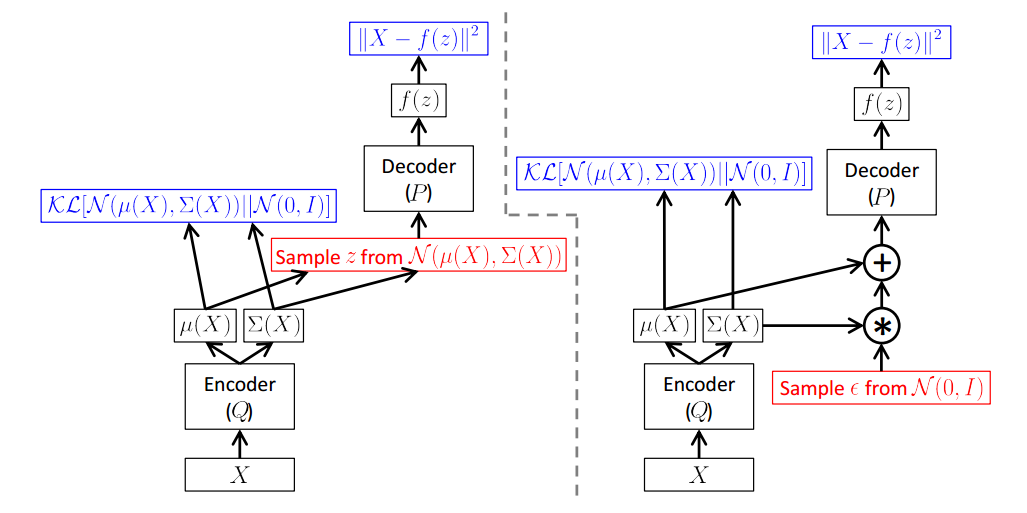
\includegraphics[scale=0.4]{images/trucoReparametrizacion.png}
\caption{(Izquierda) Modelo de VAE sin Truco de Reparametrizaci�n. (Derecha) Modelo de VAE con Truco de Reparametrizaci�n}
\label{fig:repara_trick}
\end{figure}

\par Para garantizar el correcto funcionamiento del VAE es necesario que la funci�n codificadora ($f$) asociada a $Q(z|X)$ generare un conjunto $Z$ capaz de ser decodificado por la funci�n generadora ($g$) asociada a $P(X|z)$.
\par Analizando el problema desde otra perspectiva, tomando como referencia el diagrama de izquierda de la figura \ref{fig:repara_trick}. El paso hacia delante\footnote{En el �mbito de las redes neuronales se denomina paso hacia delante (del ing�s \textit{forward pass}) al proceso incial de evaluar la salida generada a partir de una determinada entrada. En nuestro caso la entrada es $X$ y la salida $f(z)$, siendo la evaluaci�n realizada $||X - f(z)||$} funciona de manera de correcta y es de esperar (si los par�metros est�n correctamente entrenados) que la salida produzca un salida acertada de manera general. 
\par No obstante, es necesario realizar el paso hacia atr�s\footnote{En el �mbito de las redes neuronales, el paso hacia atr�s (del ingl�s \textit{backpropagation}) hace referencia al proceso de evaluar el gradiente en cada uno de los elementos del sistema, tomando como referencia que el error se?a el determinado del paso hacia delante} teniendo que determinar el gradiente sobre la funci�n $Q(z|X)$ encargada de generar $z$, pero este modelo de generaci�n esta basado en el mapeo sobre una distribuci�n gausiana, lo cual es una funci�n no continua.

\par La soluci�n a este problema se denomica truco de reparametrizaci�n (del ingl�s \textit{reparameterization trick}) el cual se basa en trasladar el mapeo sobre la distribuci�n gausiana a una capa de entrada. 
\par Dados $\mu_{X}$ y  $\Sigma_{X}$, media y convarianza respectivamente de $Q(z|X)$, podemos mapear $N(\mu_{X}, \sigma(X))$ tomando un valor de la funci�n Normal ($\epsilon \sim N(0,I)$) y aplicando la siguiente expresi�n:
\begin{center}
\begin{equation} \label{eq:RT_1}
z = \mu(X) + \Sigma(X)^{1/2} * \epsilon. 
\end{equation}
\end{center}

\par Por lo tanto la funci�n final, la cual queda representada en el diagrama de la derecha de la figura  \ref{fig:repara_trick}, sobre la que se aplica el gradiente es la siguiente:

 \begin{align}
 \begin{split}
E_{X\sim Z}\left[E_{\epsilon\sim N(0,I)}[log(P(X|z = \mu(X) + \Sigma^{1/2} * \epsilon))] - D[Q(z|X) || P(z)]\right].
\end{split} 
 \end{align}  \label{eq:RT_2}

\par Cabe notar que ninguna de las esperanzas son con respecto a las distribuciones caracter�sticas del sistema (ni $P(X|z)$ ni $Q(z|X)$) lo que nos permite realizar el gradiente sin ning�n problema sobre los elementos contenidos dentro de los valores esperados, ya que el gradiente es la derivada sobre los par�metros funcionales de estas distribuciones.
\par Por lo tanto dado un valor de $X$ y $\epsilon$ la funci�n \ref{eq:RT_2} ser� continua y determinista sobre los par�metros de $P$ y $Q$, lo cual nos permite realzar el paso hacia atr�s de manera eficaz. 
 
 
\subsection{Interpretaci�n de la funci�n objetivo} 


\begin{figure}[htp]
\centering
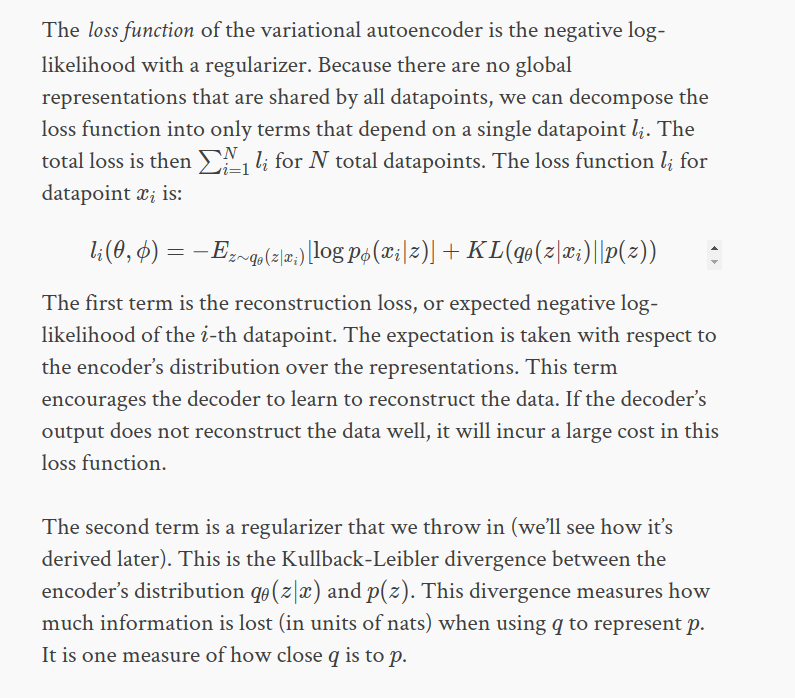
\includegraphics[scale=0.25]{images/FO_interpretacion_2.png}
\caption{Traducir }
\end{figure}


\begin{figure}[htp]
\centering
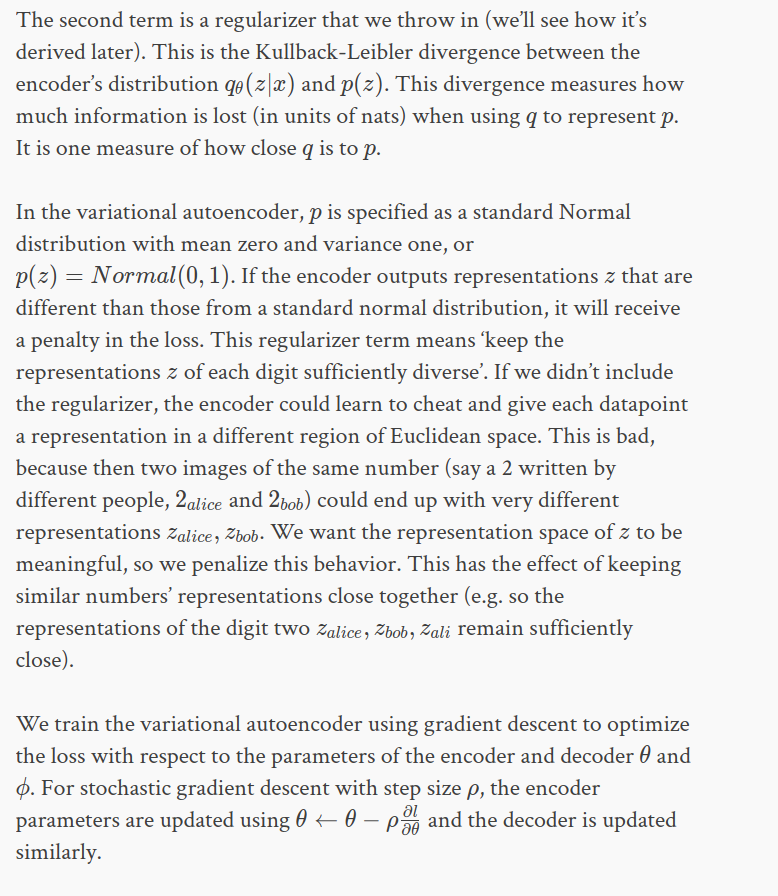
\includegraphics[scale=0.25]{images/FO_interpretacion_1.png}
\caption{Traducir }
\end{figure}


 
\subsection{Codificaci�n y Decodificaci�n}

\par La eficacia y tratabildad del m�todo reside en la asunci�n de que $Q(z|X)$, la funci�n coficadora, puede ser modelada como una gaussiana con una media determinada $\mu(X)$  y varianza $\Sigma(X)$, por otro lado es necesario que $P(X)$ converja de manera eficaz a la distribuci�n real de los datos del espacio $D$. Estas condiciones solo son superadas si y solo si $D[Q(z|X) || P(z|X)]$ es cercana a cero.
\par Es por ello necesario una funci�n $Q$ de alta capacidad, lo cual puede llevarnos a modelos complejos. Los modelos basados en funciones usados en los VAE son las redes neuronales


\begin{figure}[htp]
\centering
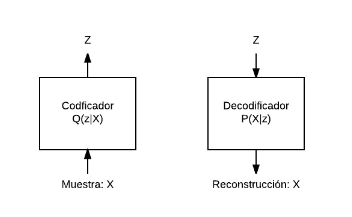
\includegraphics[scale=0.7]{images/decodificador,codificador.png}
\caption{Esquematizaci�n simple de las funciones del Codificador y el Decodificador en el VAE}
\label{fig:CD_1}
\end{figure}

\par El codificador es una red neuronal. Su entrada es el dato $X$ y su salida es la representaci�n latente $z$. Representa la distribuci�n de probabilidad $Q(z|X)$, y esta determinada por el conjunto de par�metros y pesos de la red neuronal asociada. Denominaremos a la funci�n encargada de la codificaci�n $q_{\theta}(z|x)$
\par El codificador se identifica a menudo con el proceso de reducci�n de la dimensionalidad de $x$ a $z$. Cabe notar que el codificador tiene asociadas dos funciones, una encargada de obtener la media $q_{\mu}(X)$  y otro la varianza $q_{\Sigma}(X) $ del espacio latente. Para la obtenci�n final de $z$ se ha de aplicar  el truco de reparametrizaci�n, ver seccion \ref{sec:repa_1}, con respecto a los valores $\Sigma$ y $\mu$ obtenidos anteriormente.

\par El decodificador es otra red neuronal. Su entrada es la variable del espacio latente $z$ y su salida es la reconstrucci�n del dato inicial $X$. Denominaremos a la funci�n encargada de la decodificaci�n $p_{\phi}(x|z)$, donde $\phi$ son el conjunto de par�metros y pesos que definen la red neuronal.

\par El hecho de que ambas funciones est�n basadas en redes neuronales hace el aprendizaje profundo sea una parte primordial del VAE. T�picamente los formatos de redes neuronales aplicados en este sistema son dos; redes neuronales densas (DNN)  o redes neuronales convolucionales (CNN).

\newpage
\section{Redes Neuronales}
\par Las Redes Neuronales permiten generar funciones complejas no lineales gracias a su capacidad inherente de aprendizaje con el proceso denomiado propagaci�n hacia atr�s, que permiten ajustar los pesos de las distintas unidades o neuronas del sistema. 
\par Dada la complejidad del �mbito del aprendizaje profundo, en las siguiente seciones se pretenden exponer las ideas fundamentales para comprender el comportamiento de las funciones de codificacion y decodificaci�n del VAE, sin entrar en explicaciones excesivamente te�ricas sobre los fundamentos de las redes neuronales. 
\par Es por ello que en primer lugar se expondr� el modelo de redes neuronales densas, aprovechando para exponer de manera somera algunos conceptos de redes neuronales, como son el concepto de funciones de activaci�n o el proceso de propagaci�n hacia atr�s. 

\par Seguidamente se expondr� el otro modelo de aprendizaje profundo utilizado en este trabajo que son las redes neuronales convolucionales, explcando por que son ideales para la captura de patrones sobre im�genes. 

\subsection{Red Neuronal Densa}
\par Este modelo constituye el paradigma b�sico de redes neuronales. Fundamentado en el est�ndar de neuronal artificial  seg�n los principios descritos Rumelhart y McClelland en 1986 \cite{DNN_1}. Siguiendo dichos principios, la i-�sima neurona artificial  consiste en:

\begin{figure}[!hb]
\centering
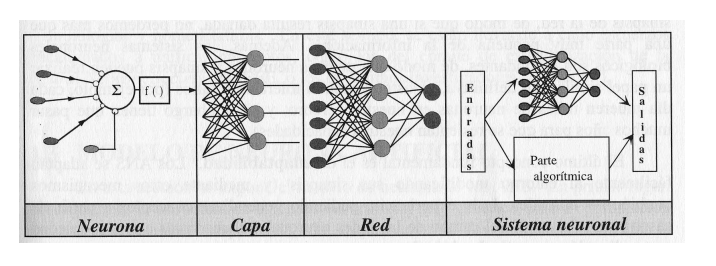
\includegraphics[scale=0.5]{images/DNN_1.png}
\caption{Sistema global de proceso de una red neuronal}
\label{fig:CD_1}
\end{figure}


\begin{itemize}

\item Un conjunto de entradas $x_j$ con un conjunto de pesos sin�pticos asociados $w_{ij}$, con $j=1,2...n$
\item Una regla de propagaci�n $h_i$ a definida partir del conjunto de entradas  y de los pesos sin�pticos. Normalmente la regla de propagaci�n utilizada el producto lineal entre los pesos sin�pticas y las entradas. Esto es:
\begin{center}
\begin{equation}\label{eq:DNN_1}
h_i(x_1,.....,x_m, w_{i1}....,w{in} = \sum_{i=1}^{n}w_{ij}*x_{j}
\end{equation}
\end{center}

\item Una funci�n de activaci�n, la cual representa simult�neamente la salida de la neurona y su estado de activaci�n. Denotando por $y_i$ dicha funci�n de activaci�n:

\begin{center}
\begin{equation} \label{eq:DNN:2}
y_i = f_i(h_i) = f_i(\sum_{j=0}^{n}w_{ij}x_{j})
\end{equation}
\end{center}  

\end{itemize} 

\subsubsection{Funci�n de Activaci�n}
\begin{figure}[!b]
\centering
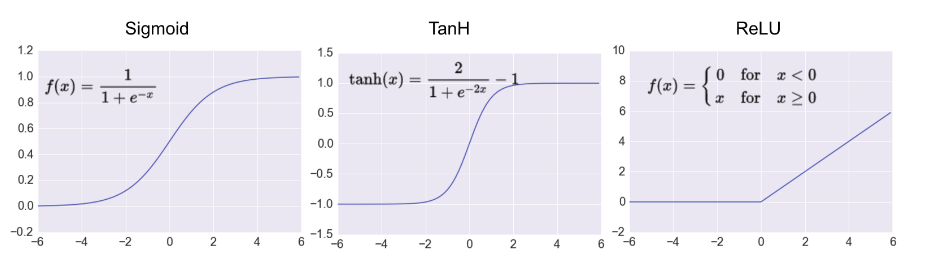
\includegraphics[scale=0.45]{images/functions_activations.png}
\caption{Principales funciones de activaci�n.}
\label{fig:CD_1}
\end{figure}
\par La eleccion de la funci�n de activaci�n constituye una parte determinante en el dise�o de redes neuronales, dado que afectar� en gran medida al a capacidad de decisi�nd de la red y la rapidez con que la red sea capaz de converger durante el entrenamiento \cite{FA_1}. 
\par En general el principal requerimiento sobre estas funciones es que sean capaces de respetar el proceso del propagaci�n hacia atr�s, no provocando que el gradiente se haga cero lo cual repercutir�a negativamente en el proceso del descenso en gradiente. Este es uno de los problemas asociadas a la clasica funci�n sigmoide, dado que para valores de $x$ ampliamente negativos o positivos, provoca que el gradiente sea cero\footnote{Este efecto es conm�nmnte denominado como saturaci�n}, interrumpiendo el descenso en gradiente para la neurona en cuesti�n y, por tanto, la optimizaci�n de sus pesos sin�pticos.



\begin{figure}[!hb]
\centering
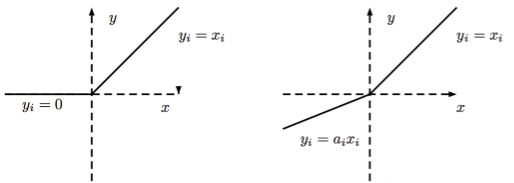
\includegraphics[scale=0.45]{images/lrelu_2.png}
\caption{(izquierda) Funci�n de activaci�n \textit{Relu}. (Derecha) Funci�n de activaci�n \textit{leakyRelu.} }
\label{fig:CD_2}
\end{figure}

\par Actualmente la funci�n de activaci�n m�s utilizada es la unidad lineal de rectificaci�n \cite{FA_2} (ReLu del ingl�s \textit{Rectifier Linear Unit}), representada en la figura \ref{fig:CD_1}. No obstante, otro tipo de funci�n de activaci�n basada en la anteriomente expuesta  denominada unidad lineal de rectificacion con p�rdidas (leakyRelu) ha ganado peso en el �mbito. La �nica diferencia entre ambas funciones es la capacidad de la \textit{leakyRelu} de no hacer nulo el gradiente para valores negativos, ver figura \ref{fig:CD_2} para apreciar esta diferencia. En este proyecto han sido utilizadas tanto la funcion Sigmoide como la funci�n \textit{leakyRelu}


\subsubsection{Topolog�a de Conexionado}
\begin{figure}[!h]
\centering
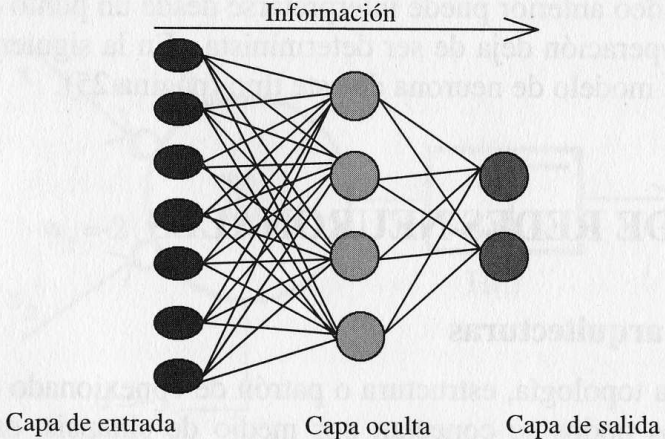
\includegraphics[scale=0.4]{images/capas.png}
\caption{Esquema de una red neuronal densa de una sola capa oculta }
\label{fig:DNN_4}
\end{figure}


\par Otro concepto determinante en el comportamiento de las redes neuronales es la topolog�a empleada, esto es, el patron de conexionado de una red neuronal. En una red neuronal artificial los nodos se conectan entre s�, siendo este conjunto de conexiones internas junto con los pesos sin�pticos lo que determina el comportamiento de la red y, en �ltima instancia, la funci�n asociada  a la red. 
\par Las unidades neuronales suelen agruparse en lo que se denominan capas. La uni�n de dos o m�s capas constituyen una red neuronal. Se distinguen tres tipos de capas: de entrada, de salida y ocultas. Una capa de entrada esta compuesta por las neuronas que reciben las se�ales. Una capa de salida est� constituida por el conjunto de neurones que proporcionan la respuesta de la red. Las capas ocultas no tienen conexionado con el exterior. A m�s capas Socultas m�s capacidad de aprendizaje tendr� el sistema, aunque el tiempo necesario para su optimizaci�n aumentar� considerablemente. 


\subsubsection{Propagaci�n Hacia Atr�s}

Se denomina propagaci�n hacia atr�s al proceso empleado para el entrenamiento de las redes neuronales. Este entrenamiento tiene como objetivo el ajuste de los pesos sin�pticos de la red. Se considera un buen ajuste de pesos aquel que minimiza el error a la salida de una red \cite{DNN_training}. De manera breve los principales pasos de este proceso de entrenamiento son:



\begin{figure}[b!]
\centering
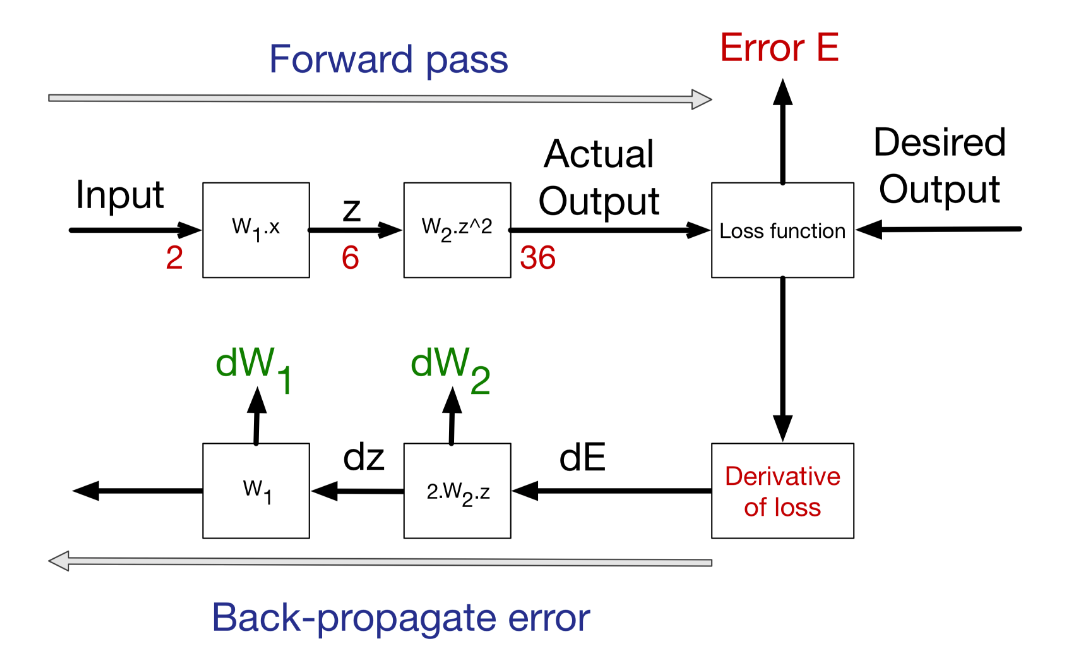
\includegraphics[scale=0.30]{images/entrenamiento.png}
\caption{Representaci�n esquem�tica del proceso de entrenamiento de una red neuronal }
\label{fig:DNN_5}
\end{figure}

\begin{itemize}
\item Inicializaci�n. Se asigna un valor por defecto a los distintos pesos. Se considera un paso determinante, puesto que una mala inicializaci�n puede implicar la saturaci�n de los gradientes en los nodos.
\par Los siguientes pasos constituyen un proceso iterativo, durante el cual se ir� minimizando progresivamente el error asociado a la salida de la red. 
\item Paso hacia delante  (\textit{Fast Forward}). Se comprueba el comportamiento de la red, se calcula la salida de la red para un conjunto de muestras de entrada. 
\item Estimaci�n del error de salida. Dada una salida, se eval�a la diferencia con respecto a la salida esperada seg�n las muestras de entrada. 
\item Se realiza la propagaci�n hacia atr�s. Dado el error a la salida se realizan el conjunto de derivadas necesarias recorriendo desde la salida hacia la entrada la red, identificando el comportamiento del gradiente del error con respecto a los diferentes pesos de la red.
\item Se modifican los pesos en funci�n del gradiente previamente calculado. 

\end{itemize}



\newpage
\subsection{Red Neuronal Convolucional}

\par Las redes convolucionales (CNN, del ingl�s \textit{Convolutional Neural Networks}) son una categor�a de redes neuronales que se consideran un m�todo altamente eficaz en �reas como el reconocimiento de im�genes \cite{CNN_1}\cite{CNN_2}.
\begin{figure}[]
\centering
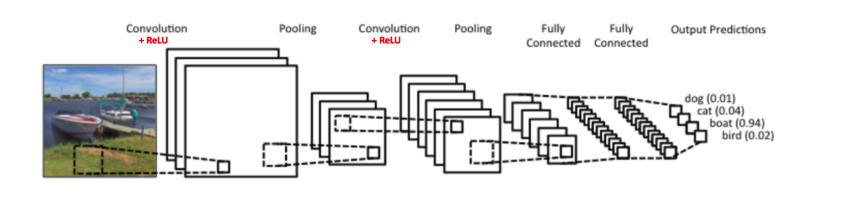
\includegraphics[scale=0.50]{images/convNet.png}
\caption{Red convolucional \textit{LeNet5} }
\label{fig:CNN_1}
\end{figure}


\par Este modelo fu� introducido en 1989 \cite{CNN} por Yann leCunn, la red de este trabajo fue denominada \textit{LeNet5}. Dicha red se puede observar en la imagen \ref{fig:CNN_1}
\par Las redes convoluciones suelen ser aplicadas a las im�genes. Cada imagen puede ser representada por una matriz de n�meros s� se trata de una imagen en escala de grises, o por tres matrices s� es una imagen a color. Es esta propiedad de las im�genes donde cada dimensi�n, es decir cada pixel, queda definida espacialmente con respecto al resto de dimensiones, lo que convierte a las im�genes en las muestras ideales para este tipo de red. 
\par Se asume que los conjuntos de pixeles vecions formar�n unas caracter�sticas m�s significativas que s� tomaramos grupos sin tener en cuenta su disposici�n espacial

a capa anterior lo que se emplea es el operador de convoluci�n.
\begin{figure}[b]
\centering
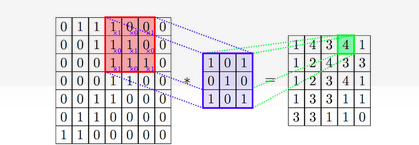
\includegraphics[scale=0.60]{images/conNet_2.png}
\caption{Ejemplo de aplicaci�n del operador convoluci�n sobre una imagen. Seleccionada una regi�n de la imagen cuyas dimensiones son las mismas que las del kernel seleccionado, se aplica el producto pixel a pixel entre dicha regi�n y los pesos propios del kernel. La suma de estos productos se almacena en la imagen de salida, respetando la ubicaci�n espacial de la regi�n evaluada. }
\label{fig:CNN_2}
\end{figure}

\par Este tipo de redes derivan su nombre del operador de red convoluci�n cuyo objetivo es extraer caracter�sticas de las im�genes preservando la relaci�n espacial entre pixeles.  

\par Dada una imagen bidimensional \textit{I} y una  matriz $K$ de dimensiones $h\times w$ (denominada kernel de convoluci�n) la cual es capaz de extraer alg�n tipo de caracter�stica relevante. La operaci�n de convoluci�n se puede representar como:  


\par Formalmente, se puede expresar como: 
\begin{center}
\begin{equation} \label{eq:CNN_2}
(I*K):{xy} = \sum_{i=1}^{h}\sum_{j=1}^{w} K_{ij}I_{I_{x+i-1},u+j-1}
\end{equation}
\end{center}  
 
\par A diferencia de las redes neuronales convencionales en las redes convolucionales los datos a la entrada y entre el conexionado de capas se agrupan en 3 dimensiones: ancho, alto y profundidad. En este caso nos referimos a "profundidad" por capa no a la profundidad de la red, lo cual se refiere al n�mero de capas  de la red en cuesti�n. Por ejemplo, dada una imagen de entrada de tres canales (los tres canales de color) de 32x32 pixeles, la agrupaci�n de los datos en la capa de entrada ser� 32x32x3. Ver figura \ref{fig:CNN_3}
\par Otra diferencia con respecto a la redes neuronales cl�sicas es que las unidades de una capa solo est�n conectadas a un espacio reducido de unidades de la capa inmediatamente anterior. 

\begin{figure}[t]
\centering
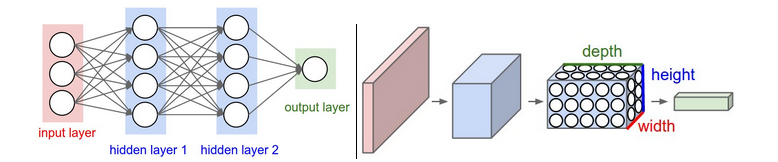
\includegraphics[scale=0.60]{images/convNet_3.png}
\caption{(Izquierda) Modelo clasico de redes neuronales. (Derecha) Modelo de Red Convolucional. Los datos son reagrupados en 3 dimensionados como se puede observar en una de las capas. Cada una de las capas tiene como entrada una imagen 3D y tiene como salida otra imagen 3D. La capa roja representa la capa de entrada por lo que la altura y la anchura son las dimensiones de la imagen y la profundidad son el n�mero de canales}
\label{fig:CNN_3}
\end{figure}

\par Las redes neuronales convolucionales se fundamentan en tres principios b�sicos que son los campos receptivos locales, los pesos compartidos y el empleo de agrupaciones o \textit{pooling}

\subsubsection{Filtros Locales}

\par En una red neuronal densa, esto es, una red totalmente conectada como la de imagen \ref{fig:CNN_3} las entradas se interpretan como un conjunto "vertical" de unidades. Sin embargo, en un red convolucional es preferible organizar las unidades de entrada en forma bidimensional.
\begin{figure}[t]
\centering
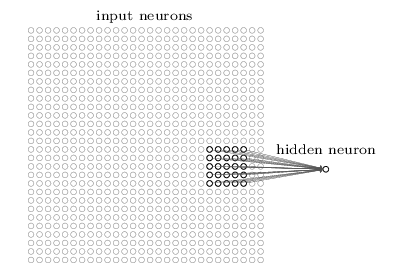
\includegraphics[scale=0.60]{images/conNet_4.png}
\caption{Representaci�n de la conectividad local en una red neuronal}
\label{fig:CNN_4}
\end{figure}

\par Las capas consecutivas estar�n conectadas entre s�, pero cada unidad de una capa oculta estar� conectada solo a un conjunto de unidades de la capa inmediatamente anterior.
\begin{figure}[b]
\centering
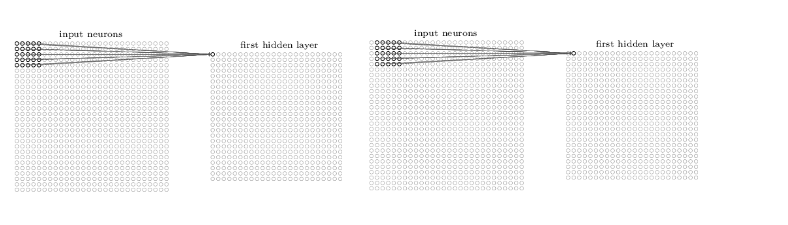
\includegraphics[scale=0.60]{images/ConvNet_6.png}
\caption{Desplazamiento del campo de recepci�n}
\label{fig:CNN_5}
\end{figure}


\par Se denomina filtro local a la ventana que se aplica a las diferentes regiones seleccionables de la imagen, cada una de estas r�giones seleccionables estan conectadas a una �nica unidad de la siguiente capa oculta. A este t�rmino a menudo nos referimos como kernel. Este filtro se desplazar� por toda la imagen, realizando el proceso de convoluci�n por toda ella, ver imagen \ref{fig:CNN_5}. Es esto lo que permite extraer caracter�sticas de manera local por toda la imagen
\par Normalmente el desplazamiento se hace pixel a pixel aunque es posible aumentar el n�mero de pixeles por desplazamiento. Este hiperpar�metro se denomina generalmente \textit{stride}. En este trabajo se ha utilizado un valor de dos. Otro concepto a tener en cuenta es que por lo general hay varios tipos de fitros para la extracci�n de caracter�sticas en las diferentes capas.  

\subsubsection{Pesos Compartidos}

\par Cada uno de los filtros de recepci�n ser�n aplicados a toda la imagen con el mismo peso para todas las diferentes regiones. Esto significa que el patr�n de selecci�n de caracter�sticas ser� el mismo, por lo que las neuronas de la siguiente capa detectar�n el mismo tipo de caracter�stica. 
\par El punto anterior se fundamente en que generalmente un patr�n  de una parte de la imagen es probable que se repita en otra parte de la imagen dada la propia naturaleza de las im�genes. 
\par Con objeto de no limitar cada capa a la extracci�n de un tipo de caracter�sticia se aplican numeros filtros en cada una de las capas de convoluci�n. Gracias a esto se consiguen extraer distintos tipos de patrones. 

\begin{figure}[t]
\centering
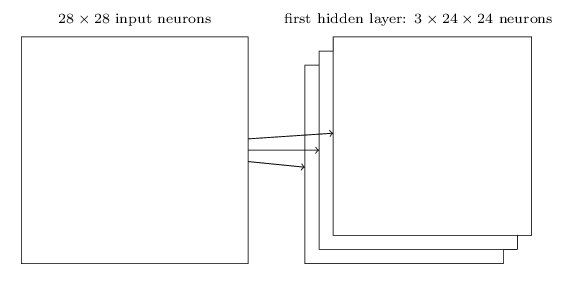
\includegraphics[scale=0.40]{images/conv_net7.png}
\caption{Representaci�n de la extracci�n de varias caracter�sticas con varios filtros}
\label{fig:CNN_6}
\end{figure}
\par Una de la ventajas del uso de pesos compartidos es que permite reducir el n�mero de par�metros de la red. 


\begin{figure}[t]
\centering
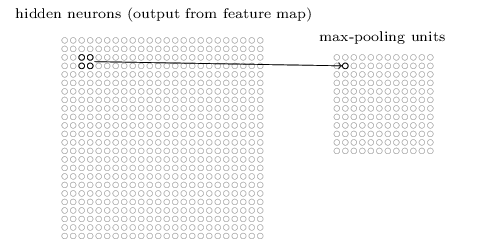
\includegraphics[scale=0.50]{images/convNet_7.png}
\caption{Representaci�n del proceso de agrupamiento (\textit{pooling})}
\label{fig:CNN_}
\end{figure}

\subsubsection{Agrupamiento}

\par Otro tipo de capa caracter�stica de las redes convolucionales son las capas de agrupamiento o \textit{pooling}.  Esta capa tiene como objetivo reducir el n�mero de datos generado, realizando una estimaci�n del valor m�s importante de una determinada region. Esto permite reducir progresivamente el tama�o de la imagen. Este proceso de agrupamiento se aplica individualmente a cada una de las imagnenes generadas por cada filtro.  
\par No obstante, esta funcionalidad no ha sido utilizada en el modelo generado en este trabajo dado que actualmente la librer�a empleada (\textit{TensorFlow})  no tiene implementada esta operaci�n para im�genes 3D. 




\newpage
\section{Herramientas Complementarias}
\subsection{M�quina de Vectores de Soporte}

\par El m�todo denominado M�quina de Vectores de Soporte (SVM, del ingl�s \textit{Support Vector Machine}) ha sido ampliamento usado para la clasificaci�n y regresi�n, dise�ado para la separaci�n de un conjunto binario de datos, pr�viamente etiquetados, mediante un hiperplano, ver figura \ref{fig:SVM_1}. 

\begin{figure}[htb]
\centering
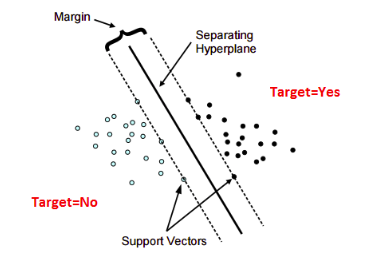
\includegraphics[scale=0.50]{images/svm_margin.png}
\caption{Representaci�n de la separaci�n binaria realizada por SVM}
\label{fig:SVM_1}
\end{figure}

\par Espec�ficamente

\newpage
\subsection{Validaci�n Cruzada (K-fold)}
\subsection{M�tricas de Validaci�n}







































\chapterend{}
%%%%%%%%%%%%%%%%%%%%%%%%%%%%%%%%%%%%%%%%%%%%%%%%%%%%%%%%%%%%%%%%%%%
%%% Documento LaTeX 																						%%%
%%%%%%%%%%%%%%%%%%%%%%%%%%%%%%%%%%%%%%%%%%%%%%%%%%%%%%%%%%%%%%%%%%%
% T�tulo:		Cap�tulo 2
% Autor:  	Ignacio Moreno Doblas
% Fecha:  	2014-02-01
% Versi�n:	0.5.0
%%%%%%%%%%%%%%%%%%%%%%%%%%%%%%%%%%%%%%%%%%%%%%%%%%%%%%%%%%%%%%%%%%%
\chapterbegin{Fundamentos Te�ricos}
\label{chp:Utiliz}
%\minitoc
\section{Estudio basado en r�giones}
fasdf
\newpage
\section{Procesado de Neuroim�genes}
sadfasdf
\newpage
\section{Modelos Generativos}
asddfasdf
\newpage
\section{Modelos de Clasificaci�n}
asdfasdf






































\chapterend{}
%%%%%%%%%%%%%%%%%%%%%%%%%%%%%%%%%%%%%%%%%%%%%%%%%%%%%%%%%%%%%%%%%%%
%%% Documento LaTeX 																						%%%
%%%%%%%%%%%%%%%%%%%%%%%%%%%%%%%%%%%%%%%%%%%%%%%%%%%%%%%%%%%%%%%%%%%
% T�tulo:		Cap�tulo 2
% Autor:  	Ignacio Moreno Doblas
% Fecha:  	2014-02-01
% Versi�n:	0.5.0
%%%%%%%%%%%%%%%%%%%%%%%%%%%%%%%%%%%%%%%%%%%%%%%%%%%%%%%%%%%%%%%%%%%
\chapterbegin{Resultados}
\label{chp:Resultados}


\section{Clasificaci�n}

\subsubsection{M�tricas de Evaluaci�n}

\par Hay diferentes m�tricas de evaluaci�n referidas a las caracter�stiscas del diagn�stico. Algunas se utilizan para evaluar la capacidad discriminativa de la prueba y otras para estimar su propiedad de predicci�n, siendo esta �ltima muy sensible a las caracter�sticas de las poblaciones evaluadas. 
\par Con objeto de valorar la calidad del test de diagn�stico es necesario saber cu�n buena y confiable es una prueba. Esta cuantificaci�n es llevada por el conjutno de medidas que se explicar�n a continuaci�n, las cu�les est�n basadas en los �ndices expuestos en la tabla \ref{table:metrics}.


\begin{table}[]
\centering
\label{table:metrics}
\begin{tabular}{C{3cm}C{3cm}|C{3cm}|C{3cm}|}
\cline{3-4}
  &  & \multicolumn{2}{c|}{	\textbf{Condici�n Real}} \\ 
\cline{3-4} 
  &  & \textbf{Positivo} & \textbf{Negativo} \\ 
\hline
\multicolumn{1}{|c|}{\multirow{2}{*}{\textbf{Predicci�n}}} & \textbf{Positivo} &  Verdadero Positivo (VP)                 &               Falso    Positivo (FP) \\ \cline{2-4} 
\multicolumn{1}{|c|}{}                            & \textbf{Negativo}     &  Falso Negativo (FN)               & Verdadero Negativo (VN)              \\ \hline
\end{tabular}
\caption{Tabla de Nomenclatura Estad�stica en Clasificaci�n}
\end{table}

\subsubsection{Medida F}

\begin{center}
\begin{equation} \label{eq:p_x_gausiana}
Valor-F = \frac{*VP}{2*VP + FP + FN}
\end{equation}
\end{center}


\subsubsection{Recall. Sensibilidad}
\par La precisi�n mide la capacidad de una prueba diagn�stica de identificar los sujetos enfermos con respecto al total de sujetos enfermos de la poblaci�n.

\begin{center}
\begin{equation} \label{eq:p_x_gausiana}
Precision = \frac{VP}{VP + FN}
\end{equation}
\end{center}


\subsubsection{Especificidad. Precisi�n}
\par La especificidad hace referencia a la capaciad de la prueba a identificar a los sujetos enfermos y excluir a aquellos que  no lo est�n. 
\begin{center}
\begin{equation} \label{eq:p_x_gausiana}
Precision = \frac{VP}{VP + FP}
\end{equation}
\end{center}

\subsubsection{Precision. Accuracy}
\par Indica la capacidad la del m�todo de clasificaci�n de identificar tanto pacientes sanos como pacientes enfermos con respecto al total de la poblaci�n.
\begin{center}
\begin{equation} \label{eq:p_x_gausiana}
F1 = \frac{VP + VN}{N�Samples}
\end{equation}
\end{center}

\subsubsection{Curva ROC}
La curva ROC (del ingl�s \textit{Receiver Operating Characteristic}) es una t�cnica gr�fica que
nos permite evaluar la precisi�n del modelo estad�stico para clasificar dos clases, AD y
NOR. La curva se obtiene calculando la sensibilidad (proporci�n de resultados positivos
verdaderos) y la especificidad del modelo en cada punto de corte posible, y trazando la
sensibilidad frente a 1-especificidad (proporci�n de resultados falsos positivos).

\par Cada punto en el espacio ROC muestra el equilibrio entre la sensibilidad y la
especificidad, es decir, que el aumento de sensibilidad va acompa�ado de una disminuci�n en la especificidad. 

\begin{figure}[!hb]
\centering
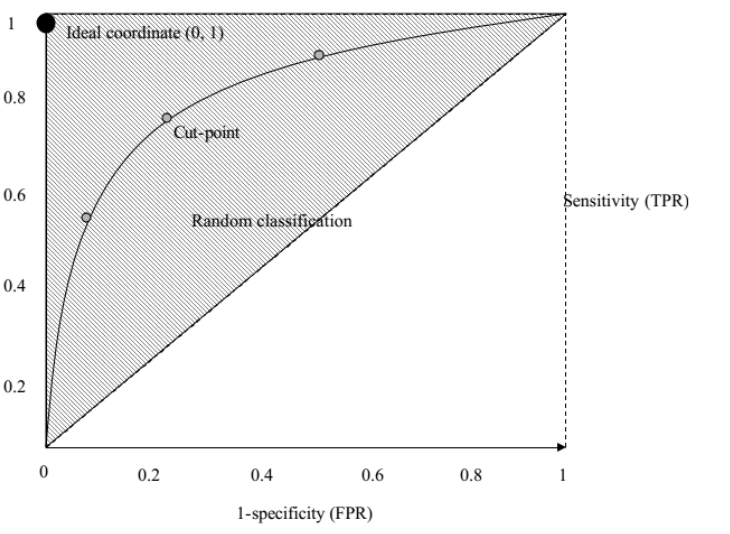
\includegraphics[scale=0.5]{images/curva_roc.png}
\caption{Representaci�nd de la curva ROC}
\label{fig:curva_roc}
\end{figure}


\par Cada punto de corte de una prueba de diagn�stico define un �nico punto en el
espacio ROC, los diferentes puntos posibles definen la curva ROC. Esto es an�logo a lo dicho para un solo punto, por tanto cuanto m�s se acerquen los puntos de la curva ROC a la coordenada ideal, m�s exacta ser� la prueba y viceversa, cuanto m�s se aleje peores
resultados obtendremos.
\subsubsection{�rea bajo la curva}

\par El �rea bajo la curva ROC se denomina AUC (del ingl�s \textit{area under the curve}) y se interpreta como el promedio de precisiones positivas y negativas. Este �ndice es especialmente �til en los estudio
comparativo de pruebas de diagn�stico. Siendo deseable comparar toda la curva ROC
en lugar de en un punto particular. 

\subsection{Resultados Clasificaci�n}


\begin{figure}[!hb]
\centering
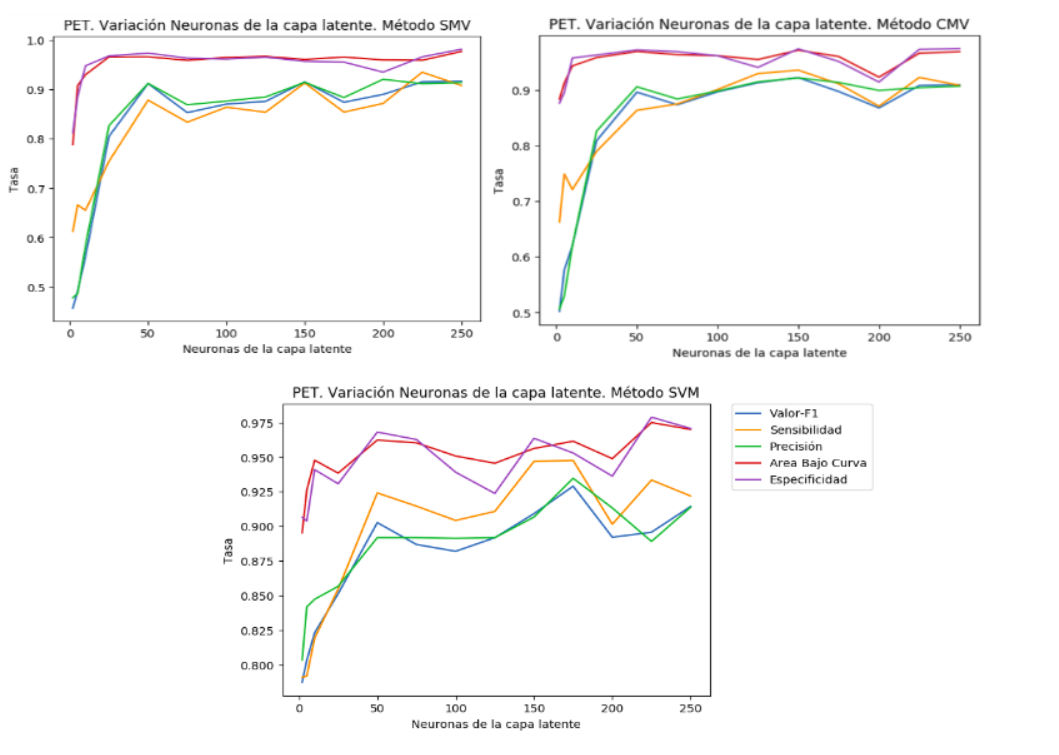
\includegraphics[scale=0.45]{images/SweepLatentLayerPET.png}
\caption{Representaci�nd de la curva ROC}
\label{fig:curva_roc}
\end{figure}

%\minitoc
\chapterend{}
\chapterbeginx{Conclusiones y l�neas futuras}

\par En este trabajo se ha analizado la t�cnica generativa denominada Autoencoder Variacional realiz�ndose dos implementaciones Software de dicha t�cnica utilizando el lenguaje \textit{Python}. Esta modelo de aprendizaje no supervisado est� basado en aprendizaje profundo, es por ello que se ha empleado la librer�a \textit{Tensorflow} que da soporte a la implementaci�n de redes neuronales para su ejecuci�n tanto en CPU como en GPU. Algunos de los aspectos a destacar, as� como algunas de las contribuciones realizadas durante el desarrollo del trabajo son las siguientes:

\begin{itemize}

\item Se ha implementado un modelo de VAE basado en redes neuronales densas. El modelo es facilmente configurable tanto en variables de configuraci�n como es la tasa de aprendizaje o en par�metros estructurales como son el n�mero de capas del modelo o el n�mero de neuronas para cada capa.

\item Se ha implementado un modelo de VAE basado en redes neuronales convolucionales. En este caso las variables de configuraci�n son modificables f�cilmente, y se han habilitado una serie de modelos que habilitan la posibilidad de selecionar entres distintas estructuras para el sistema.

\par Esta capacidad  para variar  tanto los par�metros del modelo como ciertos aspectos estructurales permite evaluar difentes configuraciones con objeto de obtener la �ptima. 

\item Se ha evaluado la capacidad de los modelos implementados de discernir entre pacientes AD y NOR emplenado tanto muestras PET como MRI. 
\par Para las imagenenes MRI se ha obtenido una precisi�n  m�xima de clasificaci�n de hasta el 84 \% para el VAE. En otros estudios, emple�ndose este mismo espacio muestral se han conseguido resultados superiores al 90 \%, por lo que son bastante superiores a los conseguidos en este trabajo. No obstante el objetivo no era conseguir un clasificador �ptimo que consiguiera competir con los modelos actuales sino demostrar la capacidad de discernir entre las neuroimagenes de un sujeto NOR y las de uno AD.
\par Para las im�genes PET se ha obtenido una precisi�n m�xima en torno al 90 \%. De nuevo estos resultados no compiten con los modelos del estado del arte actual que ronda el 95 \% con este mismo espacio muestral.

\item El objetivo principal del trabajo era conseguir realizar la s�ntesis de neuroim�genes 3D a partir de la caracterizaci�n del VAE. No obstante, las s�ntesis realizadas utilzando el c�digo generado por las propias im�genes del espacio muestral han generado unas im�genes que apenas se asemejaban a las originales. 
\par Tanto para el modelo VAE de redes densas como para el CVAE se ha tenido un resultado nefasto para la s�ntesis aunque hay diversos aspectos en la implementaci�n de ambos modelos que son diferentes. Esto genera la duda de si el problema est� en la implementaci�n del modelo o en el m�todo VAE en s� que no se ajuste al objetivo de este trabajo. 
\par En las simulaciones de visualizaci�n del c�digo latente se ha comprobado como es posible separar para algunas regiones el c�digo generado para im�genes de sujetos AD y para sujetos NOR. Esto nos indica que el autoencoder es capaz de generar un c�digo diferente para los dos tipos de sujetos. Sin embargo durante la fase de reconstrucci�n se tiene que los c�digos generan de nuevo el mismo tipo de imagen. Una imagen final que puede representar un valor medio de imagen que permite reducir el error de regeneraci�n durante el proceso de entrenamiento.
\par En resumen, es realmente desconcertante que c�digos latentes diferenciables entre NOR y AD generen finalmente un mismo tipo de imagen, o al menos muy similar. 

\item Otro aspecto importante es que el uso de redes convolucionales 3D como modelo extracci�n de caracter�sticas para el VAE no es una metodolog�a que se haya usado en muchos trabajos relativos a esta tem�tica, al menos durante la fase inicial de este proyecto no se encontro ning�n c�digo de implementaci�n sobre \textit{Tensorflow} de este tipo de red. Adem�s, \textit{Tensorflow} no dispone de la funci�n encargada de realizar el proceso de agrupamiento (\textit{pooling}) para im�genes 3D, lo cu�l puede conlleva la imposibilidad de probar esta funcionalidad de reducci�n de caracter�sticas en el sistema. 

\subsection{L�neas futuras}
\par En este trabaja la implementaci�n se ha apoyado en \textit{Tensorflow} para la realizaci�n de los dise�os. Existen diversas librer�as sobre \textit{Python} que facilitan el mismo conjunto de funcionalidades que \textit{Tensorflow}, tales librer�as son \textit{Keras} o \textit{Theano}, es por ello que una posible l�nea de trabajo ser�a realizar la implementaci�n sobre alguna de estas librer�a y evaluar si los resultados de la s�ntesis de im�genes son similares. Esto nos permitir�a descartar si los problemas de este trabajo son debidos a las implementaciones aqu� realizadas.

\par Adem�s de VAE, existen otros tipos de t�cnicas generativas que se basan en el uso de aprendizaje profundo. Las redes generativas adversarias, que fueren brevemente comentadas en la secci�n \ref{sec_redesAdversarias}, constituyen un m�todo caracterizado por generar una s�ntesis de im�genes m�s realista que el VAE pero que es ciertamente m�s complejo de entrenar y de llegar a una configuraci�n �ptima de los par�metros. 
\end{itemize}

\chapterend

% Cap�tulo 04.
%\input{Capitulo04.tex}

\appendix

%%%%%%%%%%%%%%%%%%%%%%%%%%%%%%%%%%%%%%%%%%%%%%%%%%%%%%%%%%%%%%%%%%%
%%% Documento LaTeX 																						%%%
%%%%%%%%%%%%%%%%%%%%%%%%%%%%%%%%%%%%%%%%%%%%%%%%%%%%%%%%%%%%%%%%%%%
% T�tulo:		Ap�ndice A
% Autor:  	Ignacio Moreno Doblas
% Fecha:  	2014-02-01
% Versi�n:	0.5.0
%%%%%%%%%%%%%%%%%%%%%%%%%%%%%%%%%%%%%%%%%%%%%%%%%%%%%%%%%%%%%%%%%%%%

\pagestyle{fancy}
\fancyhead[LE,RO]{\thepage}
\fancyhead[RE]{Ap�ndice} %
\fancyhead[LO]{\nouppercase{\rightmark}}
%\fancyhead[RE]{Parte \thepart \rightmark} %

\chapter{Ap�ndice}

\minitoc

\section{Primera secci�n}
 
 Manejadores de datos


Benchmark


\begin{itemize}
\item Un script para los dos tipo de imagenes  es facil de manipular
\item Loop over latent-layer

\item threshold definitions

\item Container to store evaluation information


\item timing evaluataion, neural net behaviour

\item cv\_utils created to generate differente kfolds samples distribution in each iteration over a feature

\item Support over not convergin regions in cvae

\item SVM diferente para cada tipo de imagen

\item Loading data:
\item PET
\item MRI  GM/WM

\item Session Description
\end{itemize}


\chapterend

%\input{D2.AppendixB.tex}

%\input{D3.AppendixC.tex}

% Formato de documento en la parte final.
\backmatter
%Hace que los cap�tulos y t�tulos nivel inferior no aparezcan numerados (lo que es ideal para conclusiones o notas finales).

% Bibliograf�a
%%%%%%%%%%%%%%%%%%%%%%%%%%%%%%%%%%%%%%%%%%%%%%%%%%%%%%%%%%%%%%%%%%%%
%%% Documento LaTeX 																						%%%
%%%%%%%%%%%%%%%%%%%%%%%%%%%%%%%%%%%%%%%%%%%%%%%%%%%%%%%%%%%%%%%%%%%
% Título:		Bibliografía
% Autor:  	Ignacio Moreno Doblas
% Fecha:  	2014-02-01
% Versión:	0.5.0
%%%%%%%%%%%%%%%%%%%%%%%%%%%%%%%%%%%%%%%%%%%%%%%%%%%%%%%%%%%%%%%%%%%%

% Encabezamiento %
\pagestyle{fancy}
\fancyhead[LE,RO]{\thepage}
\fancyhead[LO]{Bibliografía}
%\fancyhead[RE]{Parte \thepart \rightmark} %
\fancyhead[RE]{\nouppercase{\rightmark}} %

%Inclusión de bibliografía%

%Inclusión en el índice (Tabla de contenidos)

%Formateo de estilo de bibliografía
% Otros formatos: plain, unsrt, abbrv
%  plain: las entradas se ordenan alfabéticamente y se etiquetan con un número (p.ej., [1])
% unsrt: igual que plain, pero aparecen en orden de citación.
% alpha: el etiquetado se hace por autor y año de publicación (p.ej., [Knu66]).
% abbrv: igual que alpha, pero más abreviado.
\begin{thebibliography}{9}

\bibitem{Alzheimer1} 
	Henley, David B.,
	Sundell, Karen L.,
	Sethuraman, Gopalan,
 	Siemers, Eric R.,
	2011,	
	\textit{Safety profile of Alzheimer's disease populations in Alzheimer's Disease Neuroimaging 			Initiative and other 18-month studies},
 	407-416

\bibitem{ReservaCognitiva}
	Rodríguez Álvarez M., Sánchez J. L.,
	2004,
	\textit{Reserva cognitiva y demencia},
	2004, vol. 20, nº 2 (diciembre), 175-186 
	
\bibitem{DiagnosticoNormal}
 Petrella J.R, Coleman R.E., Doraiswamy P.M., Neuroimaging and Early Diagnosis
of Alzheimer Disease: A Look to the Future. Radiology 2003; 226:315?336.



\bibitem{MRIsurvey}
	Rémi Cuingnet et al, 
	\textit{Automatic classification of patients with Alzheimer's disease from
	structural MRI: A comparison of ten methods using the ADNI database},
	 Neuroimage,
	vol. 56, no. 2, pp. 766-781, 2011.

\bibitem{introPET}
	W. Cai, 
	D. Feng, 
	R. Fulton, 
	\textit{Content-based retrieval of dynamic PET functional images} 
	IEEE Trans. Inf. Technol. Biomed., vol. 4, no. 2, pp. 152-158, 2000.

\bibitem{PETMRIMultimodal}
	Ortiz, A.; 
	Fajardo, D.; 
	Górriz, J.M.; 
	Ramírez, J.; 
	Martínez-Murcia, F.J.,
	\textit{Multimodal
image data fusion for Alzheimer's Disease diagnosis by sparse representation}, 
International Conference on Innnovation in Medicine and Healthcare (InMed), 2014


\bibitem{PETMRIMultimodal2}
	Daoqiang Zhanga, 
	Yaping Wanga, 
	Luping Zhoua, 
	Hong Yuana, 
	Dinggang Shena,
	\textit{Multimodal Classification of Alzheimer's Disease and Mild Cognitive Impairment}
	Neuroimage. 2011 April 1; 55(3): 856-867


\bibitem{SVMtrees}
	D. Salas-Gonzalez, 
	J. M. Gorriz, 
	J. Ramírez, 
	M. Lopez, 
	I Alvarez,
	\textit{Compute-aided diagnosis of Alzheimer's disease using support vector machines and classification trees}
	Phys. Med. Biol. 55 (2010) 2807-2817


\bibitem{Survey}
	Ruaa Adeeb Abdulmunem Al-falluji
	\textit{MRI based Techniques for Detection of Alzheimer: A Survey}
	International Journal of Computer Applications (0975 - 8887)
	Volume 159 - No 5, February 2017

\bibitem{Survey2}
	S.Mareeswari1, 
	Dr.G.Wiselin,
	\textit{A survey Early Detection of Alzheimer's Disease using different techniques}
	International Journal on Computational Science and Applications (IJCSA) Vol.5, No.1,February 2015

\bibitem{CoD}
Bellman RE, 
1961,
\textit{Adaptive control processes: a guided tour}, Princeton
University Press.


\bibitem{CoD2}
	David L. Donoho
	Department of Statistics
	\textit{High-Dimensional Data Analysis: The Curses and Blessings of Dimensionality}
	August 8, 2000

\bibitem{ReduceDimensionality}
	Benson Mwangi, 
	Tian Siva Tian,  
	Jair C. Soares
	\textit{A review of feature reduction techniques in neuroimaging}
	Neuroinformatics. 2014 April ; 12(2): 229-244. doi:10.1007/s12021-013-9204-3.

\bibitem{DeepLearning1}
	Siqi Liu, 
	Sidong Liu,
	\textit{EARLY DIAGNOSIS OF ALZHEIMER'S DISEASE WITH DEEP LEARNING}

\bibitem{DeepLearning2}
	Saman S., 
	Ghassem T.,
	\textit{Classification of Alzheimer's Disease Structural MRI Data by Deep Learning Convolutional Neural Networks}
	22 Jul 2016

\bibitem{AutoEncoderVariational}
	Diederik P. Kingma,
	Max Welling,
	\textit{Auto-Encoding Variational Bayes}
	1 May 2014

\bibitem{AutoEncoderOrigin1}
	 D. E. Rumelhart, G. E. Hinto, and R. J. Williams. 
	 Learning Internal Representations by Error Propagation
	 9 October 1986

\bibitem{AutoEncoderSurvey}
	: I. Guyon, 
	G. Dror, 
	V. Lemaire, 
	G. Taylor and 
	D. Silver
	Autoencoders, Unsupervised Learning, and Deep Architectures
	2012

\bibitem{AutoEncoderDenoising}
	P. Vincent
	H. Larochelle
	I. Lajoie
	Stacked Denoising Autoencoders: Learning Useful Representations in a Deep Network with a Local Denoising Criterion
	2010

\bibitem{VAE_gen}
ADVERSARIAL EXAMPLES FOR GENERATIVE MODELS

\bibitem{DeepGenerativeModels}
	Danilo J. Rezende, 
	Shakir Mohamed, 
	Daan Wierstra
	Stochastic Backpropagation and Approximate Inference in Deep Generative Models

\bibitem{AD_historic}
	Bennett, D. A.,
	Evans, D. A., 
	1922.
	Alzheimer's Disease.
	Disease-a-Month 38(1), 7-64.

\bibitem{ADhistoric2}
	Nakako, S.,
	Kato, T.,
	Nakamura.,
	1996.
	Acetylcholinesterase activity in cerebrospinal fluid of patients with alzhimer's disease and senile dementia.
	Journal of the Neurological Sciences
	75(2).
\bibitem{mitocondria2}
	Rodriguez-Violante M.,
	Cervantes A.,
	Vargas S.,
	2010.
	Papel de la función mitocondrial en las enfermedades neurodegenerativas.
	Arch Neurocien (Mex)  Vol. 15, Nº1: 39-46

\bibitem{mitocondriaGeneral}
	Swerdlow, R.,
	2011
	Brain agin, alzheimer's diseas, and mitochondira.
	Biochim Biophys Acta 1812(12), 1630-1639


\bibitem{Nations}
	Nations U.,
	2008
	Department of economic and social affairs, world population prospects. 

\bibitem{Predemencia1}
	 Arnáiz E,., 
	 Almkvist O., 
	 2003,. 
	 Neuropsychological features of mild cognitive impairment and preclinical Alzheimer's disease. 



\bibitem{Predemencia2}
 	Palmer K., 
 	Berger A. K., 
 	Monastero R., 
 	Winblad B., 
 	Bäckman L., 
 	Fratiglioni L. 
 	2007. 
 	Predictors of progression from mild cognitive impairment to Alzheimer disease. 
 	Neurology 68 (19): 1596-1602. 
 	PMID 17485646. doi:10.1212/01.wnl.0000260968.92345.3f.

\bibitem{DemenciaMemoria}
	 Carlesimo GA, Oscar-Berman M (junio de 1992). «Memory deficits in Alzheimer's patients: a comprehensive review». Neuropsychol Rev 3 (2): 119-69. PMID 1300219.

 \bibitem{DemenciaComunicacion}
 	 Frank EM (septiembre de 1994). «Effect of Alzheimer's disease on communication function». J S C Med Assoc 90 (9): 417-23. PMID 7967534.
\bibitem{ADconducta}
	Volicer L, 
	Harper DG, 
	Manning BC, 
	Goldstein R, 
	Satlin A., 
	Mayo de 2001. 
	Sundowning and circadian rhythms in Alzheimer's disease». Am J Psychiatry 158 (5): 704-711. PMID 11329390. 


\bibitem{hipocampo}
	Mu Y., 
	Gage FH,
	2011 Dec,
Mol Neurodegener. 2011 Dec 22;6:85. doi: 10.1186/1750-1326-6-8
Adult hippocampal neurogenesis and its role in Alzheimer's disease.


\bibitem{atlasAlzheimer}
	FeldMan H. H.,
	Atlas of Alzheimer's Disease.
	Informa Healthcare

\bibitem{MainADNI}
	Susanne G. Mueller, 
	Michael W. Weiner, 
	Neuroimaging Clin N Am. 2005 November ; 15(4): 869–xii.
	The Alzheimer’s Disease Neuroimaging Initiative
	
\bibitem{}
 Gorji, H. T.; Haddadnia, J. (2015-10-01). "A novel method for early diagnosis of Alzheimer's disease based on pseudo Zernike moment from structural MRI". Neuroscience. 305: 361–371. ISSN 1873-7544. PMID 26265552. doi:10.1016/j.neuroscience.2015.08.013.

\bibitem{}
 Zhu, Xiaofeng; Suk, Heung-Il; Shen, Dinggang (2014-10-15). "A novel matrix-similarity based loss function for joint regression and classification in AD diagnosis". NeuroImage. 100: 91–105. ISSN 1095-9572. PMC 4138265 Freely accessible. PMID 24911377. doi:10.1016/j.neuroimage.2014.05.078.


\end{thebibliography}




%Impresión de todas las entradas bibliográficas
\nocite{*}

\chapterend
%\begin{thebibliography}{9}

\bibitem{Alzheimer1} 
	Henley, David B.,
	Sundell, Karen L.,
	Sethuraman, Gopalan,
 	Siemers, Eric R.,
	2011,	
	\textit{Safety profile of Alzheimer's disease populations in Alzheimer's Disease Neuroimaging Initiative and other 18-month studies},
 	407-416


\bibitem{ReservaCognitiva}
	Rodríguez Álvarez M., Sánchez J. L.,
	2004,
	\textit{Reserva cognitiva y demencia},
	2004, vol. 20, nº 2 (diciembre), 175-186 
	
\bibitem{DiagnosticoNormal}
 Petrella J.R, Coleman R.E., Doraiswamy P.M., Neuroimaging and Early Diagnosis
of Alzheimer Disease: A Look to the Future. Radiology 2003; 226:315?336.



\bibitem{MRIsurvey}
	Rémi Cuingnet et al, 
	\textit{Automatic classification of patients with Alzheimer's disease from
	structural MRI: A comparison of ten methods using the ADNI database},
	 Neuroimage,
	vol. 56, no. 2, pp. 766-781, 2011.

  \end{thebibliography}


\begin{thebibliography}{9}

\bibitem{Alzheimer1} 
	Henley, David B.,
	Sundell, Karen L.,
	Sethuraman, Gopalan,
 	Siemers, Eric R.,
	2011,	
	\textit{Safety profile of Alzheimer's disease populations in Alzheimer's Disease Neuroimaging 			Initiative and other 18-month studies},
 	407-416

\bibitem{ReservaCognitiva}
	Rodr�guez �lvarez M., S�nchez J. L.,
	2004,
	\textit{Reserva cognitiva y demencia},
	2004, vol. 20, n� 2 (diciembre), 175-186 
	
\bibitem{DiagnosticoNormal}
 Petrella J.R, Coleman R.E., Doraiswamy P.M., Neuroimaging and Early Diagnosis
of Alzheimer Disease: A Look to the Future. Radiology 2003; 226:315?336.

\bibitem{MRIsurvey}
	R�mi Cuingnet et al, 
	\textit{Automatic classification of patients with Alzheimer's disease from
	structural MRI: A comparison of ten methods using the ADNI database},
	 Neuroimage,
	vol. 56, no. 2, pp. 766-781, 2011.

\bibitem{introPET}
	W. Cai, 
	D. Feng, 
	R. Fulton, 
	\textit{Content-based retrieval of dynamic PET functional images} 
	IEEE Trans. Inf. Technol. Biomed., vol. 4, no. 2, pp. 152-158, 2000.

\bibitem{PETMRIMultimodal}
	Ortiz, A.; 
	Fajardo, D.; 
	G�rriz, J.M.; 
	Ram�rez, J.; 
	Mart�nez-Murcia, F.J.,
	\textit{Multimodal
image data fusion for Alzheimer's Disease diagnosis by sparse representation}, 
International Conference on Innnovation in Medicine and Healthcare (InMed), 2014


\bibitem{PETMRIMultimodal2}
	Daoqiang Zhanga, 
	Yaping Wanga, 
	Luping Zhoua, 
	Hong Yuana, 
	Dinggang Shena,
	\textit{Multimodal Classification of Alzheimer's Disease and Mild Cognitive Impairment}
	Neuroimage. 2011 April 1; 55(3): 856-867


\bibitem{SVMtrees}
	D. Salas-Gonzalez, 
	J. M. Gorriz, 
	J. Ram�rez, 
	M. Lopez, 
	I Alvarez,
	\textit{Compute-aided diagnosis of Alzheimer's disease using support vector machines and classification trees}
	Phys. Med. Biol. 55 (2010) 2807-2817


\bibitem{Survey}
	Ruaa Adeeb Abdulmunem Al-falluji
	\textit{MRI based Techniques for Detection of Alzheimer: A Survey}
	International Journal of Computer Applications (0975 - 8887)
	Volume 159 - No 5, February 2017

\bibitem{Survey2}
	S.Mareeswari1, 
	Dr.G.Wiselin,
	\textit{A survey Early Detection of Alzheimer's Disease using different techniques}
	International Journal on Computational Science and Applications (IJCSA) Vol.5, No.1,February 2015

\bibitem{CoD}
Bellman RE, 
1961,
\textit{Adaptive control processes: a guided tour}, Princeton
 University Press.


\bibitem{CoD2}
	David L. Donoho
	Department of Statistics
	\textit{High-Dimensional Data Analysis: The Curses and Blessings of Dimensionality}
	August 8, 2000

\bibitem{ReduceDimensionality}
	Benson Mwangi, 
	Tian Siva Tian,  
	Jair C. Soares
	\textit{A review of feature reduction techniques in neuroimaging}
	Neuroinformatics. 2014 April ; 12(2): 229-244. doi:10.1007/s12021-013-9204-3.

\bibitem{DeepLearning1}
	Siqi Liu, 
	Sidong Liu,
	\textit{EARLY DIAGNOSIS OF ALZHEIMER'S DISEASE WITH DEEP LEARNING}

\bibitem{DeepLearning2}
	Saman S., 
	Ghassem T.,
	\textit{Classification of Alzheimer's Disease Structural MRI Data by Deep Learning Convolutional Neural Networks}
	22 Jul 2016

\bibitem{AutoEncoderVariational}
	Diederik P. Kingma,
	Max Welling,
	\textit{Auto-Encoding Variational Bayes}
	1 May 2014

\bibitem{AutoEncoderOrigin1}
	 D. E. Rumelhart, G. E. Hinto, and R. J. Williams. 
	 Learning Internal Representations by Error Propagation
	 9 October 1986

\bibitem{AutoEncoderSurvey}
	: I. Guyon, 
	G. Dror, 
	V. Lemaire, 
	G. Taylor and 
	D. Silver
	Autoencoders, Unsupervised Learning, and Deep Architectures
	2012

\bibitem{AutoEncoderDenoising}
	P. Vincent
	H. Larochelle
	I. Lajoie
	Stacked Denoising Autoencoders: Learning Useful Representations in a Deep Network with a Local Denoising Criterion
	2010

\bibitem{VAE_gen}
ADVERSARIAL EXAMPLES FOR GENERATIVE MODELS

\bibitem{DeepGenerativeModels}
	Danilo J. Rezende, 
	Shakir Mohamed, 
	Daan Wierstra
	Stochastic Backpropagation and Approximate Inference in Deep Generative Models

\bibitem{AD_historic}
	Bennett, D. A.,
	Evans, D. A., 
	1922.
	Alzheimer's Disease.
	Disease-a-Month 38(1), 7-64.

\bibitem{ADhistoric2}
	Nakako, S.,
	Kato, T.,
	Nakamura.,
	1996.
	Acetylcholinesterase activity in cerebrospinal fluid of patients with alzhimer's disease and senile dementia.
	Journal of the Neurological Sciences
	75(2).
\bibitem{mitocondria2}
	Rodriguez-Violante M.,
	Cervantes A.,
	Vargas S.,
	2010.
	Papel de la funci�n mitocondrial en las enfermedades neurodegenerativas.
	Arch Neurocien (Mex)  Vol. 15, N�1: 39-46

\bibitem{mitocondriaGeneral}
	Swerdlow, R.,
	2011
	Brain agin, alzheimer's diseas, and mitochondira.
	Biochim Biophys Acta 1812(12), 1630-1639


\bibitem{Nations}
	Nations U.,
	2008
	Department of economic and social affairs, world population prospects. 

\bibitem{Predemencia1}
	 Arn�iz E,., 
	 Almkvist O., 
	 2003,. 
	 Neuropsychological features of mild cognitive impairment and preclinical Alzheimer's disease. 



\bibitem{Predemencia2}
 	Palmer K., 
 	Berger A. K., 
 	Monastero R., 
 	Winblad B., 
 	B�ckman L., 
 	Fratiglioni L. 
 	2007. 
 	Predictors of progression from mild cognitive impairment to Alzheimer disease. 
 	Neurology 68 (19): 1596-1602. 
 	PMID 17485646. doi:10.1212/01.wnl.0000260968.92345.3f.

\bibitem{DemenciaMemoria}
	 Carlesimo GA, Oscar-Berman M (junio de 1992). �Memory deficits in Alzheimer's patients: a comprehensive review�. Neuropsychol Rev 3 (2): 119-69. PMID 1300219.

 \bibitem{DemenciaComunicacion}
 	 Frank EM (septiembre de 1994). �Effect of Alzheimer's disease on communication function�. J S C Med Assoc 90 (9): 417-23. PMID 7967534.
\bibitem{ADconducta}
	Volicer L, 
	Harper DG, 
	Manning BC, 
	Goldstein R, 
	Satlin A., 
	Mayo de 2001. 
	Sundowning and circadian rhythms in Alzheimer's disease�. Am J Psychiatry 158 (5): 704-711. PMID 11329390. 


\bibitem{hipocampo}
	Mu Y., 
	Gage FH,
	2011 Dec,
Mol Neurodegener. 2011 Dec 22;6:85. doi: 10.1186/1750-1326-6-8
Adult hippocampal neurogenesis and its role in Alzheimer's disease.


\bibitem{atlasAlzheimer}
	FeldMan H. H.,
	Atlas of Alzheimer's Disease.
	Informa Healthcare

\bibitem{MainADNI}
	Susanne G. Mueller, 
	Michael W. Weiner, 
	Neuroimaging Clin N Am. 2005 November ; 15(4): 869?xii.
	The Alzheimer?s Disease Neuroimaging Initiative
	
\bibitem{}
 Gorji, H. T.; Haddadnia, J. (2015-10-01). "A novel method for early diagnosis of Alzheimer's disease based on pseudo Zernike moment from structural MRI". Neuroscience. 305: 361?371. ISSN 1873-7544. PMID 26265552. doi:10.1016/j.neuroscience.2015.08.013.

\bibitem{}
 Zhu, Xiaofeng; Suk, Heung-Il; Shen, Dinggang (2014-10-15). "A novel matrix-similarity based loss function for joint regression and classification in AD diagnosis". NeuroImage. 100: 91?105. ISSN 1095-9572. PMC 4138265?Freely 
 accessible. PMID 24911377. doi:10.1016/j.neuroimage.2014.05.078.

\bibitem{MRIOrigin3}
Wright G., 
Magnetic Resonance Imaging
EEE Signal Process. Mag. 14 (1997)56?66.


\bibitem{MRIOrigin}
Lauterbur P. C., 1973. 
"Image Formation by Induced Local Interactions: Examples of Employing Nuclear Magnetic Resonance". 
Nature. 242 (5394): 

\bibitem{MRIOrigin2}
 "Britain's brains produce first NMR scans". 
 New Scientist: 588. 1978.

\bibitem{MRINoise}
Snehal More, 
V.V.Hanchate,
"A Survey on Magnetic Resonance Image Denoising Methods"
International Research Journal of Engineering and Technology (IRJET),
Volume: 03 Issue: 05 | May-2016 

\bibitem{rbm}
Asja Fischer,
Christian Igel,
\textit{An Introduction to Restricted Boltzmann Machines}


\bibitem{denoising_autoencoder}
Vincent H.,
Larochelle H.,
Lajoie. I.,
\textit{Stacked Denoising Autoencoders: Learning Useful Representations in
a Deep Network with a Local Denoising Criterion}

\bibitem{denoising_autoencoder2}
Vincent, Pascal
Larochelle, Hugo
Bengio, Yoshua
\textit{Extracting and Composing Robust Features with Denoising Autoencoders},
  (ICML'08), pages 1096 - 1103, 2008

\bibitem{gan}
 Goodfellow, Ian J.; 
 Pouget-Abadie, Jean; 
 Mirza, Mehdi; 
 Xu, Bing; 
 Warde-Farley, 
 David; Ozair, 
 Sherjil; Courville, 
 Aaron; Bengio, Yoshua 
 (2014), 
 "Generative Adversarial Networks". arXiv:1406.2661?

\bibitem{gan_example}
Salimans T., 
Goodfellow I., 
Zaremba., 
Cheung, Vicki; Radford, Alec; Chen, Xi (2016).
"Improved Techniques for Training GANs". arXiv:1606.03498?



\bibitem{vae_2d}
Eunbyung Park 
University of North Carolina at Chapel Hill


\bibitem{mri_survey}
\textit{MRI based Techniques for Detection of Alzheimer: A
Survey} 
Ruaa Adeeb Abdulmunem Al-falluji
University of Babylon,
International Journal of Computer Applications (0975 ? 8887),
Volume 159 ? No 5, February 2017
\bibitem{ica}

Yang, Wenlu, et al. "Independent component analysis-
based classification of Alzheimer's disease MRI
data." Journal of Alzheimer's disease 24.4 (2011): 775-
783.

\bibitem{pca}
18F-FDG PET imaging analysis for computer aided
Alzheimer?s diagnosis? I.A. Ill�n, J.M. G�rriz,J.
Ram�rez, D. Salas-Gonzalez, M.M. L�pez, F. Segovia,
R. Chaves, M. G�mez-Rio c, C.G. Puntonet,
Information Sciences 181 903?916, 2011.

\bibitem{wavelet}

Herrera, Luis Javier, et al. "Classification of MRI
Images for Alzheimer's Disease Detection." Social
Computing
(SocialCom),
2013
International
Conference on. IEEE, 2013.


\bibitem{knn}

Zhang, H., Berg, A.C., Maire, M., Svm-knn, J.M.:
Discriminative nearest neighbor classification for visual
category recognition. In: CVPR ?06, pp. 2126?2136.
IEEE Computer Society, Los Alamitos, CA, USA
(2006)

\bibitem{deep_learning}
Weiner, Michael (2017). "Recent publications from the Alzheimer's disease neuroimaging initiative: reviewing progress toward improved AD clinical trials.". Alzheimer's and dementia.


\bibitem{deep_learning_2}
 Suk, Heung-Il; Lee, Seong-Whan; Shen, Dinggang; Alzheimer?s Disease Neuroimaging Initiative (2016-06-01). 
 "Deep sparse multi-task learning for feature selection in Alzheimer's disease diagnosis". 

\bibitem{deep_learning_3}

 Zu, Chen; Jie, Biao; Liu, Mingxia; Chen, Songcan; Shen, Dinggang; Zhang, Daoqiang; Alzheimer?s Disease Neuroimaging Initiative (2016-12-01). "Label-aligned multi-task feature learning for multimodal classification of Alzheimer's disease and mild cognitive impairment". Brain Imaging and Behavior.

\bibitem{cnn_ad_1}
Hosseini-Asl E., 
Keynton R., 
El-Baz A.,
\textit{Alzheimer?s disease diagnostics by adaptation of 3d convolutional network}
(Julio 2016), 
arXiv:1607


\bibitem{cnn_ad_2}
Suk H-I., 
Shen D., 
\textit{Deep Learning-Based Feature Representation for AD/MCI Classification}, 
Medical image computing and computer-assisted intervention?(MICCAI), International Conference on Medical Image Computing and Computer-Assisted Intervention. 2013;16(0 2):583-590.

\bibitem{tensorflow}
Abadi M, 
Agarwal A., 
Barham P., 
B. Eugene,. 
\textit{TensorFlow:
Large-Scale Machine Learning on Heterogeneous Distributed Systems}, 
November 9, 2015

\bibitem{DNN_1}
D.E. Rumelhart, J.L. MacClelland (eds.) (1986). Parallel Distributed Processing.
Vol 1. Foundations, MIT Press

\bibitem{FA_1}
Glorot, X.,
Bengio, Y.,
(2010).
\textit{Understanding the difficulty of training deep feedforward neural networks}
Journal of Machine Learning Research - Proceedings Track. 9. 249-256.  

\bibitem{FA_2}
LeCun, Yann; Bengio, Yoshua; Hinton, Geoffrey (2015). "Deep learning". Nature. 521 (7553): 436?444. Bibcode:2015Natur.521..436L. PMID 26017442. doi:10.1038/nature14539.

\bibitem{DNN_training}
Xavier Glorot and Yoshua Bengio,
\textit{Understanding the difficulty of training deep feedforward neural networks},
(2010)
In Proceedings of the International Conference on Artificial Intelligence and Statistics (AISTATS?10). Society for Artificial Intelligence and Statistics

\bibitem{CNN}
LeCun,  Y.,  Boser,  B.,  Denker,  J.  S.,
Backpropagation  applied  to  handwritten  zip  code
recognition.
Neural Comput.
, 1(4):541?551, 1989

\bibitem{CNN_1}
Visualizing and Understanding Convolutional Networks
Ciresan, D. C., Meier, J., and Schmidhuber, J.  Multi-
column  deep  neural  networks  for  image  classifica-
tion.  In
CVPR
, 2012.

\bibitem{CNN_2}
Krizhevsky,  A.,  Sutskever,  I.,  and  Hinton,  G.E.   Im-
agenet classification with deep convolutional neural
networks.  In
NIPS
, 2012.


\end{thebibliography}

% �ndice alfab�tico%
%%%%%%%%%%%%%%%%%%%%%%%%%%%%%%%%%%%%%%%%%%%%%%%%%%%%%%%%%%%%%%%%%%%
%%% Documento LaTeX 																						%%%
%%%%%%%%%%%%%%%%%%%%%%%%%%%%%%%%%%%%%%%%%%%%%%%%%%%%%%%%%%%%%%%%%%%
% T�tulo:		Glosario (index)
% Autor:  	Ignacio Moreno Doblas
% Fecha:  	2014-02-01
% Versi�n:	0.5.0
%%%%%%%%%%%%%%%%%%%%%%%%%%%%%%%%%%%%%%%%%%%%%%%%%%%%%%%%%%%%%%%%%%%%

\pagestyle{fancy}
\fancyhead[LE,RO]{\thepage}
\fancyhead[LO]{�ndice Alfab�tico}
%\fancyhead[RE]{Parte \thepart \rightmark} %
\fancyhead[RE]{\nouppercase{\rightmark}} %

%index of contents
\phantomsection
\addcontentsline{toc}{chapter}{�ndice alfab�tico}
\printindex


%Example 	Index Entry 	Comment
%\index{hello} 	hello, 1 	Plain entry
%\index{hello!Peter} 	  Peter, 3 	Subentry under 'hello'
%\index{Sam@\textsl{Sam}} 	Sam, 2 	Formatted entry
%\index{Lin@\textbf{Lin}} 	Lin, 7 	Same as above
%\index{Jenny|textbf} 	Jenny, 3 	Formatted page number
%\index{Joe|textit} 	Joe, 5 	Same as above
%\index{ecole@\'ecole} 	�cole, 4 	Handling of accents
%\index{Peter|see{hello}} 	Peter, see hello 	Cross-references
%\index{Jen|seealso{Jenny}} 	Jen, see also Jenny 	Same as above

\chapterend

\end{document}
